\documentclass[a4paper, twoside]{report}

%% Language and font encodings
\usepackage[portuges]{babel}
\usepackage[T1]{fontenc}
\usepackage{verbatim}
%%%%% Estes dois packages servem para mudar a fonte para Calibri, a mesma do template do professor. Demora demasiado tempo a compilar para o overleaf, portanto tem de se fazer download e compilar localmente antes de se entregar.
%%%%% \usepackage{fontspec}
%%%%% \setmainfont{Calibri}

%% Sets page size and margins
\usepackage[a4paper,top=3cm,bottom=2cm,left=3cm,right=3cm,marginparwidth=1.75cm, paperwidth=210mm,textwidth=160mm]{geometry}
%% Useful packages
\usepackage{amsmath}
\usepackage{graphicx}
\usepackage[colorinlistoftodos]{todonotes}
\usepackage[colorlinks=true, allcolors=blue]{hyperref}
\usepackage{multirow}



\title{Ginásio do Miguel}
\author{Adelino Miguel Alves Silva, A82549\\
        Henrique José Carvalho Faria, A82200\\
        Luís Filipe da Costa Cunha, A83099\\
        Miguel Ângelo Moreira Ramos Brandão, A82349}
% Update supervisor and other title stuff in title/title.tex

\usepackage{listings}
\usepackage{color}
\usepackage{rotating}

\definecolor{dkgreen}{rgb}{0,0.6,0}
\definecolor{gray}{rgb}{0.5,0.5,0.5}
\definecolor{mauve}{rgb}{0.58,0,0.82}

\lstset{frame=tb,
  language=SQL,
  aboveskip=3mm,
  belowskip=3mm,
  showstringspaces=false,
  columns=flexible,
  basicstyle={\small\ttfamily},
  numbers=none,
  numberstyle=\tiny\color{gray},
  keywordstyle=\color{blue},
  commentstyle=\color{dkgreen},
  stringstyle=\color{mauve},
  breaklines=true,
  breakatwhitespace=true,
  tabsize=3
}



\begin{document}
\begin{titlepage}

\newcommand{\HRule}{\rule{\linewidth}{0.5mm}} % Defines a new command for the horizontal lines, change thickness here

%----------------------------------------------------------------------------------------
%	LOGO SECTION
%----------------------------------------------------------------------------------------


\includegraphics[width=8cm]{title/logoEEUM.jpg}\\[1cm] % Include a department/university logo - this will require the graphicx package
 
%----------------------------------------------------------------------------------------

\center % Center everything on the page

%----------------------------------------------------------------------------------------
%	HEADING SECTIONS
%----------------------------------------------------------------------------------------

\textsc{\LARGE Universidade do Minho}\\[1.5cm] % Name of your university/college
\textsc{\Large Mestrado Integrado em Engenharia Informática\\Ciências da Computação}\\[0.5cm] % Major heading such as course name
\textsc{\large Base de Dados}\\[0.5cm] % Minor heading such as course title

%----------------------------------------------------------------------------------------
%	TITLE SECTION
%----------------------------------------------------------------------------------------
\makeatletter
\HRule \\[0.4cm]
{ \huge \bfseries \@title}\\[0.4cm] % Title of your document
\HRule \\[1.5cm]
 
%----------------------------------------------------------------------------------------
%	AUTHOR SECTION
%----------------------------------------------------------------------------------------

% \begin{minipage}{0.4\textwidth}
% \begin{flushleft} \large
% \emph{Author:}\\
% \@author % Your name
% \end{flushleft}
% \end{minipage}
% ~
% \begin{minipage}{0.4\textwidth}
% \begin{flushright} \large
% \emph{Supervisor:} \\
% Prof. Lily Smith \\[1.2em] % Supervisor's Name
% \emph{Second Marker:} \\
% Dr. Adam Smith % second marker's name
% \end{flushright}
% \end{minipage}\\[2cm]
% \makeatother

% If you don't want a supervisor, uncomment the two lines below and remove the section above
\Large 
%\emph{Autores:}
%\\
\@author\\[3cm] % Your name

%----------------------------------------------------------------------------------------
%	DATE SECTION
%----------------------------------------------------------------------------------------

{\large \today}\\[2cm] % Date, change the \today to a set date if you want to be precise

\vfill % Fill the rest of the page with whitespace

\end{titlepage}

\renewcommand{\abstractname}{Resumo}

\begin{abstract}
Este projeto consiste na criação de uma base de dados para o Sr.Miguel, o dono de um pequeno ginásio que viu um aumento exponencial no número de clientes nas últimas semanas e como tal necessitou de uma estrutura para  organizar os seus dados.\par
Com o intuito, de criar uma base de dados que satisfaça todas as necessidades requeridas pelo nosso cliente, e para que esta consiga suportar e organizar todos os dados necessários, de forma correta e moderada, foi realizada uma pesquisa exaustiva acerca do funcionamento do ginásio do senhor Miguel. Esta pesquisa consistiu em várias observações presenciais, contacto com os operários regulares do ginásio e claro, esclarecimento, com a administração do ginásio, dos principais objetivos que o ginásio pretendia alcançar com a implementação desta base de dados.\par
No final da análise presencial, e do levantamento de todos os requisitos necessários para cumprir com as expetativas do nosso cliente, começamos a desenvolver a base de dados. Inicialmente elaboramos um modelo conceptual, para confirmar se os requerimentos levantados iam ao encontro do pretendido pelo Sr.Miguel. Depois de todo o modelo estar devidamente corrigido e validado, procedemos  para a criação do modelo lógico. Aqui foi onde começamos a dar forma à estrutura lógica da base de dados. Transformamos toda a informação visual do modelo conceptual em estruturação lógica para finalmente, depois da validação e confirmação do modelo lógico, passarmos á criação do modelo Físico. Foi nesta fase que demos origem a todas as funcionalidades requeridas pelo nosso cliente. Finalmente, o cliente pode ver a base de dados em funcionamento, realizando todas as operações por ele requeridas e guardando, organizando e gerindo todos os dados do seu Ginásio.

\par Toda a metodologia utilizada ao longo do trabalho é a apresentada pelo livro "A Practical Approach toDesign, Implementation, and Management."  \cite{dbsys} 

\subsection*{Palavras Chave}
Sistema de Base de Dados Relacional, Modelo Conceptual, Modelo Lógico, Modelo Físico, Notação Peter Chen, Modelo ER, Entidades, Atributos, Relacionamentos, Java, Sistema de Base de Dados não Relacional, MySQL, NoSQL, MongoDB, SQL.

\end{abstract}

%% TODO
% verificar que está tudo direito nas tabelas de atributos e assim
%mecanismos de segurança noSQL?


\tableofcontents
\listoffigures
\listoftables
\lstlistoflistings

\part{Projeto de um Sistema de Bases de Dados Relacional}
\chapter{Definição do Sistema}
\section{Contexto da Aplicação do Sistema}

O Miguel gosta muito de fazer exercício. Ultrajado com o preço dos ginásios na sua área, ele decide investir no seu próprio equipamento e começar um pequeno ginásio pessoal. Sendo um estudante de Engenharia Informática extremamente popular entre o público feminino, começou a receber diversos pedidos das suas amigas para também poderem treinar no seu ginásio. Sabendo disto, alguns outros estudantes demonstraram interesse em treinar no ginásio do Miguel. 

\section{ Fundamentação da Implementação da Base de Dados}
 Com o aumento de clientes, o ginásio teve a necessidade de expandir as suas instalações, comprar novo equipamento e também recrutar novos funcionários, para conseguir satisfazer a necessidade dos seus clientes.
 Como tal, Miguel concluiu que era conveniente armazenar a informação detalhada dos seus funcionários e equipamentos.
 \par Com a intenção de criar um ligação mais próxima com os clientes, o Miguel intendeu que se devia guardar também a informação do cliente. Uma ação como mandar um postal pelo Natal, ou pelo aniversário e mandar mensagens para incentivar o treino era impossível sem guardar os dados dos clientes.
\section{Análise de Viabilidade do Processo}
Trata-se de um modelo genérico de um sistema de base de dados, desenvolve-se em torno de um fornecedor(O Miguel), serviço(todas as atividades possíveis desenvolver no ginásio, desde personal training a planos de nutrição) e cliente, ou seja, o processo de desenvolvimento desta base de dados é bastante simples e como tal parece-nos um sistema de base de dados fácil de implementar.

\chapter{Levantamento e análise de requisitos}

\section{Métodos de levantamento e de análise de requisitos adotados}

Durante a fase de coleta de requisitos do sistema foram usadas diversas técnicas, como a consulta de documentos utilizados (memorandos, emails, queixas de empregados face ao sistema e criticas/avaliação da performance do sistema), para perceber a origem da necessidade de uma base de dados. O dono, futuro administrador da base de dados, listou as funções que acha necessárias e deu o seu parecer acerca do funcionamento normal do ginásio. Foram realizadas entrevistas adicionais com os funcionários do estabelecimento para verificação dos requisitos já identificados, bem como clarificação dos mesmos e possíveis adições de novos requisitos que fossem de encontro às necessidades destes. Por fim, a equipa de levantamento de requisitos procedeu à coleta de dados por observação do normal funcionamento do ginásio através do sistema de vigilância, visto que o facto de um funcionário saber que está a ser observado pode interferir na forma como uma atividade é executada, e como clientes, de modo a ter uma perceção de como a base de dados poderia influenciar a experiência de um cliente.


\section{Requisitos Levantados}

\subsection{Requisitos de Descrição}

Os requisitos de descrição necessários á base de dados recolhidos pela equipa foram :

\begin{enumerate}
    \item  É necessário guardar o nome,sexo,idade, Serviço Prestado, contacto,email e Morada do funcionário. 
    \item Um Serviço é constituído por um nome e pelo respetivo preço.
    \item Temos de guardar todos os dados pessoais do cliente(nome, sexo,idade,contacto,email,morada,Número de Contribuinte) e \textit{IMC}, Peso, Altura, e Limitações Físicas.
    \item Os exercícios são compostos pelo seu tipo e nome associado ao mesmo.
    \item O equipamento tem nome e um propósito. 
    \item A fatura é composta pelo numero de contribuinte empresa, data de emissão, descrição, valor, número contribuinte do cliente, serviço prestado.
    
\item O cliente tem um conjunto de  de exercícios,que formam um plano de exercícios.

\item O plano de exercícios é composto pelo número de repetições e número de series.

\item O Cliente antes de ter acesso aos serviços fornecidos no ginásio tem de se registar nos mesmos,registando a data de subscrição.

\item O ginásio tem de ter a funcionalidade de emitir fatura dos serviços fornecidos ao cliente.

\item Após a subscrição de um ou vários serviços, é submetida uma fatura desses serviços, sendo necessário guardar essas relações para futura consulta.

\item Existem funcionários a fornecer serviços específicos.

\item Deve ser registado o momento em que o funcionário se torna responsável pela prestação do serviço.


\item O cliente tem sempre exercícios, a menos q este se subscreva a um serviço de natação ou a um serviço de nutrição, e estes últimos são sempre diferentes de pessoa para pessoa.

\item Para todo o exercício existe também um equipamento adequado para a sua execução.
\par
\end{enumerate}
\subsection{Requisitos de Exploração}
\label{subsec:requisitos}
Após a verificação das necessidades dos funcionários e do responsável do ginásio para permitir um bom funcionamento deste, chegamos às seguintes conclusões:

\begin{enumerate} 
    \item Terá de ser possível ao responsável do ginásio adicionar um funcionário.
    \item Terá também  de ser possível ao administrador do ginásio alterar a informação relativa a um funcionário;
    \item Para posterior confirmação dos updates ou adições referentes ao funcionário o administrador deverá poder visualizar o conteúdo da tabela dos funcionários.
    \item Tem de ser possível visualizar que serviços são prestados por que funcionários. 
    \item O responsável do ginásio poderá também consultar os serviços fornecidos pelo ginásio.
    \item Outra das funções do administrador do ginásio será adicionar novos serviços que poderão vir a ser disponibilizados aos clientes.
    \item Este terá também a obrigação de marcar como não disponíveis os serviços que entretanto forem descontinuados ou os quais o ginásio já não suporte.
    \item Terá de ser possível ao funcionário registar um novo cliente;
    \item Existe a necessidade de aceder à ficha do cliente pelo número de utilizador.
    \item Também deverá ser possível aceder á ficha do cliente através do seu número de telefone, caso este não saiba o seu idCliente;
    \item Terá de ser possível ao funcionário consultar os exercícios de um cliente.
    \item O funcionário deverá ter permissões para adicionar novos exercícios a um cliente.
    \item Para além disso terá de ser também disponibilizada forma de apagar os exercícios associados a um cliente do seu plano de treinos;
    \item Deverá ser possível a consulta de todas as faturas emitidas pelo ginásio relativas a um cliente.
    \item A consulta de faturas entre  duas datas específicas será também uma funcionalidade presente na base de dados;
    \item Ao funcionário reserva-se o dever de emitir faturas.
    \item Ao funcionário reserva-se também o dever de marcar uma fatura como inválida sempre que esta for mal inserida no sistema.
    \item O responsável reserva-se o dever de ter acesso ao total faturado num determinado período de tempo ou durante todo o tempo de vida do ginásio.
    \item Cabe ao funcionário designar qual o equipamento a ser utilizado num determinado exercício no momento da inserção deste na base de dados.
    \item Quer o administrador quer os rececionistas devem poder ver que serviços foram registados em cada fatura.
    \item Os funcionários devem poder também ver quais as subscrições dos clientes.
    \item No ginásio é requerida a necessidade de poder adicionar novos equipamentos, isto poderá ser feito quer pelos funcionários quer pelo administrador do ginásio.
    \item Um funcionário pode decidir adicionar um novo exercício aos atualmente disponíveis para os clientes.
    \item O administrador será responsável por referenciar que funcionários executam que serviço.
\end{enumerate}


\subsection{Requisitos de Controlo}

\begin{enumerate}
\item Horário de acesso:\par
Tanto o administrador como os funcionários podem aceder à base de dados durante o horário de funcionamento do ginásio, das 8 da manhã até á meia noite.
\item Funcionários, fornecedores e Serviços:\par
Apenas o administrador poderá consultar, adicionar ou remover dados referentes a estas entidades.
\item Cliente:\par
Um funcionário tem total acesso ao cliente podendo adicionar, remover ou modificar os dados de um cliente.
\item Equipamento:\par
Tanto o funcionário como o administrador podem alterar os dados referentes a um equipamento.
\item Exercícios:\par
Apenas o funcionário poderá adicionar, modificar ou remover um exercício.
\item Faturas:\par
Tanto o administrador como o funcionário podem consultar e alterar as faturas. Mas apenas um administrador pode remover uma.

\end{enumerate}

\section{Análise geral dos Requisitos}

Para esta base de dados realizou-se uma combinação das visões do administrador, dos funcionários e dos clientes utilizando a  \textit{Centralized aproach} pois o sistema a modelar não é muito complexo e as vistas dos utilizadores sobrepõem-se em vários aspetos. (Apesar dos clientes não operarem sobre a base de dados é importante saber as suas necessidades como obter a lista de exercícios correspondentes ao seu plano de treino)
\newline
\par
Ao realizar uma análise mais profunda dos requisitos podemos inferir que o principal interveniente do sistema é o funcionário visto que este lida com os dados dos clientes, exercícios, faturas e equipamentos do ginásio.
Podemos também verificar que a entidade central é o Cliente pois este realiza exercícios, subscreve um ou mais serviços e paga pelos mesmos.


\chapter{Modelação Conceptual}



\section{Apresentação da abordagem de modelação realizada}

A abordagem escolhida para modelar a base de dados do senhor Miguel baseai-se numa modelação conceptual, que é independente de qualquer implementação que envolva aplicações, linguagens de programação, interfaces de hardware, etc. Para isso, iremos utilizar um modelo abstrato de Entidade-Relacionamento (ER) com a notação de \textbf{Peter Chen} para elaborar um diagrama de entidades, com os seus atributos, e relacionamentos entre elas.\par
Primeiramente, fizemos o levantamento dos elementos principais do nosso modelo, as entidades. Para isso, um dos métodos que usamos foi, por exemplo, analisar os requisitos selecionando os elementos mais destacados.\par
Em segundo lugar, identificamos de que forma as entidades anteriormente selecionadas se relacionam entre si para assim, criar-mos relacionamentos entre elas. Mais uma vez, fizemo-lo  analisando as expressões usadas nos requerimentos levantados.\par
Em terceiro lugar, procedemos à identificação de atributos das entidades ou relacionamentos necessários à base de dados. Para isso identificamos caraterísticas, qualidades e propriedades das varias entidades e relacionamentos, anteriormente levantados, e selecionamos as mais relevantes para o problema em questão.\par
Em quarto lugar, identificamos, para cada atributo, o seu domínio.\par
Em quinto lugar, para cada entidade, selecionamos, entre todos os seus atributos, a melhor chave primária.\par
Seguidamente, verificamos a existência de redundância no nosso modelo, ou seja, analisamos entidade a entidade de forma a confirmar que não tínhamos entidades repetidas, depois focamo-nos nos relacionamentos para garantir que todos eles são imperscindiveis, ou seja, existe pelo menos um caso em que apenas aquele relacionamento me poderia dar acesso àquela informação.\par
Finalmente, procedemos á validação de todo o modelo ao lado do senhor Miguel.

\section{Identificação e caracterização das entidades}
Para identificarmos as várias entidades do nosso modelo conceptual, uma das abordagens tomadas foi a análise rigorosa dos requerimentos levantados. Nomes principais referentes a um ginásio ou objetos os quais sejam bastantes referidos  ou detalhados nos requerimentos feitos pelo senhor Miguel tendem a ser bons candidatos a entidades. \par
Para além disso, procuramos ter em atenção entidades auto suficientes, ou seja, entidades que existem por si próprias, independentes de qualquer outra entidade. Exemplo disso é a entidade Funcionário, pois esta existe, independentemente de sabermos quem são, a sua idade, ou o seu cargo.
Nesta fase, consideramos que a participação e acompanhamento do senhor Miguel foi essencial sendo que, por vezes, foi necessário um melhor esclarecimento dos requisitos de forma a termos um modelo conceptual mais preciso.

\clearpage

\section{Identificação e caracterização dos relacionamentos}

A fim de identificar os vários relacionamentos entre a entidades já anteriormente identificadas iremos mais uma vez  recorrer à  observação dos requerimentos. Desta vez iremos adotar uma análise diferente, que consiste na observação das expressões usadas, focada nos verbos utilizados para relacionar as nossas identidades.\par
Assim, os relacionamentos que selecionamos são:
\vspace{10 pt}


\begin{table}[ht]
\centering
\resizebox{\textwidth}{!}{
\begin{tabular}{|c|c|c|c|}
\hline
Entidade    & Relacionamento      & Entidade    & Cardinalidade \\ \hline
Cliente     & Plano de Exercícios & Exercício   & (0,N) - (0,N) \\ \hline
Cliente     & Tem                 & Fatura      & (1,1) - (0,N) \\ \hline
Cliente     & Subscreve           & Serviço     & (0,N) - (1,N) \\ \hline
Funcionário & Passa               & Fatura      & (1,1) - (1,N) \\ \hline
Equipamento & É utilizado para    & Exercício   & (1,N) - (0,N) \\ \hline
Serviço     & É prestado por      & Funcionário & (0,N) - (0,N) \\ \hline
Serviço     & Constitui           & Fatura      & (1,N) - (0,N) \\ \hline
\end{tabular}
}
\end{table}
\newpage

\section{Identificação e caracterização das Associação dos Atributos
com as Entidades e Relacionamentos.}

No final de reunir todas as entidades e relacionamentos relevantes para o nosso modelo, procedemos então à identificação e caraterização de todos os atributo necessários de modo a cumprir com o requerimentos estabelecidos. Na  tabela 3.1 é possível visualizar todos os atributos de cada entidade e as caraterísticas associadas a cada um deles.

\vspace{10 pt}

\begin{table}[h]
\resizebox{\textwidth}{!}{
\begin{tabular}{|c|ccccccccc|}
\hline
\textbf{Entidade}             & \multicolumn{1}{c|}{\textbf{Atributos}}                        & \multicolumn{1}{c|}{\textbf{Descrição}}                                                                                   & \multicolumn{1}{c|}{\textbf{\begin{tabular}[c]{@{}c@{}}Chave \\ Primária\end{tabular}}} & \multicolumn{1}{c|}{\textbf{Domínio}}                                                                             & \multicolumn{1}{c|}{\textbf{\begin{tabular}[c]{@{}c@{}}Tipo de\\  dados\end{tabular}}} & \multicolumn{1}{c|}{\textbf{Nulo}} & \multicolumn{1}{c|}{\textbf{Multivalor}} & \multicolumn{1}{c|}{\textbf{Composto}} & \textbf{Derivado} \\ \hline
\multirow{17}{*}{Cliente}     & ClienteID                                                      & Identificação do cliente                                                                                                  & Sim                                                                                     & Até 5 dígitos                                                                                                     & INT                                                                                    & Não                                & Não                                      & Não                                    & Não               \\
                              & Nome                                                           & Nome do cliente                                                                                                           & Não                                                                                     & Até 75 caracteres                                                                                                 & VARCHAR(75)                                                                            & Não                                & Não                                      & Não                                    & Não               \\
                              & Idade                                                          & Idade do cliente                                                                                                          & Não                                                                                     & Até 3 dígitos                                                                                                     & INT                                                                                    & Não                                & Não                                      & Não                                    & Não               \\
                              & Morada                                                         & Morada do cliente                                                                                                         & --                                                                                      & --                                                                                                                & --                                                                                     & --                                 & Não                                      & Sim                                    & Não               \\
                              & Localidade                                                     & Localidade do cliente                                                                                                     & Não                                                                                     & Até 75 caracteres                                                                                                 & VARCHAR(75)                                                                            & Não                                & Não                                      & Não                                    & Não               \\
                              & Rua                                                            & Rua do cliente                                                                                                            & Não                                                                                     & Até 75 caracteres                                                                                                 & VARCHAR(75)                                                                            & Não                                & Não                                      & Não                                    & Não               \\
                              & Codigo Postal                                                  & Codigo Postal do Cliente                                                                                                  & Não                                                                                     & \begin{tabular}[c]{@{}c@{}}4 dígitos+\\ 1 caractere "-"+\\ 3 dígitos\end{tabular}                                 & VARCHAR(8)                                                                             & Não                                & Não                                      & Não                                    & Não               \\
                              & Contacto                                                       & Contacto do cliente                                                                                                       & --                                                                                      & --                                                                                                                & --                                                                                     & --                                 & Não                                      & Sim                                    & Não               \\
                              & Telemovel 1                                                     & Nº de telefone do cliente                                                                                                 & Não                                                                                     & 9 dígitos                                                                                                         & INT                                                                                    & Não                                & Não                                      & Não                                    & Não               \\
                              & Telemovel 2                                                     & \begin{tabular}[c]{@{}c@{}}Segundo nº de telefone do \\ cliente\end{tabular}                                              & Não                                                                                     & 9 dígitos                                                                                                         & INT                                                                                    & Sim                                & Não                                      & Não                                    & Não               \\
                              & Email                                                          & Email do cliente                                                                                                          & Não                                                                                     & Até 75 caracteres                                                                                                 & VARCHAR(75)                                                                            & Não                                & Não                                      & Não                                    & Não               \\
                              & IMC                                                            & \begin{tabular}[c]{@{}c@{}}Indice de massa corporal\\  do cliente\end{tabular}                                            & Não                                                                                     & \begin{tabular}[c]{@{}c@{}}Até 4 dígitos\\ (2 decimais)\end{tabular}                                              & DECIMAL(4,2)                                                                           & Não                                & Não                                      & Não                                    & Sim               \\
                              & Peso                                                           & Peso do cliente                                                                                                           & Não                                                                                     & \begin{tabular}[c]{@{}c@{}}Até 5 dígitos\\ (2 decimais)\end{tabular}                                              & DECIMAL(5,2)                                                                           & Não                                & Não                                      & Não                                    & Não               \\
                              & Altura                                                         & Altura do cliente                                                                                                         & Não                                                                                     & \begin{tabular}[c]{@{}c@{}}Até 4 dígitos\\ (2 decimais)\end{tabular}                                              & DECIMAL(4,2)                                                                           & Não                                & Não                                      & Não                                    & Não               \\
                              & Nr Contribuinte                                                & Nº de contribuinte do cliente                                                                                             & Não                                                                                     & 9 dígitos                                                                                                         & INT                                                                                    & Não                                & Não                                      & Não                                    & Não               \\
                              & Sexo                                                           & Sexo do cliente                                                                                                           & Não                                                                                     & 1 caractere (F/M)                                                                                                 & VARCHAR(1)                                                                             & Não                                & Não                                      & Não                                    & Não               \\
                              & Dependencias Fisicas                                           & \begin{tabular}[c]{@{}c@{}}Dependências físicas do \\ cliente\end{tabular}                                                & Não                                                                                     & Até 45 caracteres                                                                                                 & VARCHAR(45)                                                                            & Sim                                & Não                                      & Não                                    & Não               \\ \hline
\multirow{13}{*}{Funcionário} & FuncionárioID                                                  & Identificação do funcionário                                                                                              & Sim                                                                                     & Até 4 dígitos                                                                                                     & INT                                                                                    & Não                                & Não                                      & Não                                    & Não               \\
                              & Nome                                                           & Nome do funcionário                                                                                                       & Não                                                                                     & Até 45 caracteres                                                                                                 & VARCHAR(45)                                                                            & Não                                & Não                                      & Não                                    & Não               \\
                              & Cargo                                                          & \begin{tabular}[c]{@{}c@{}}Cargo que o funcionário \\ ocupa no ginásio\end{tabular}                                       & Não                                                                                     & Até 75 caracteres                                                                                                 & VARCHAR(75)                                                                            & Não                                & Não                                      & Não                                    & Não               \\
                              & Idade                                                          & Idade do funcionário                                                                                                      & Não                                                                                     & Até 3 dígitos                                                                                                     & INT                                                                                    & Não                                & Não                                      & Não                                    & Não               \\
                              & Contacto                                                       & Contacto do funcionário                                                                                                   & --                                                                                      & --                                                                                                                & --                                                                                     & --                                 & --                                       & Sim                                    & Não               \\
                              & Telemovel 1                                                     & Nº do telefone do funcionário                                                                                             & Não                                                                                     & 9 dígitos                                                                                                         & INT                                                                                    & Não                                & Não                                      & Não                                    & Não               \\
                              & Telemovel 2                                                     & \begin{tabular}[c]{@{}c@{}}Segundo nº de telefone do \\ funcionário\end{tabular}                                          & Não                                                                                     & 9 dígitos                                                                                                         & INT                                                                                    & Sim                                & Não                                      & Não                                    & Não               \\
                              & Email                                                          & Email do funcionário                                                                                                      & Não                                                                                     & Até 75 caracteres                                                                                                 & VARCHAR(75)                                                                            & Não                                & Não                                      & Não                                    & Não               \\
                              & Morada                                                         & Morada do funcionário                                                                                                     & Não                                                                                     & --                                                                                                                & --                                                                                     & --                                 & --                                       & Sim                                    & Não               \\
                              & Rua                                                            & Rua onde o funcionário habita                                                                                             & Não                                                                                     & Até 75 caracteres                                                                                                 & VARCHAR(75)                                                                            & Não                                & Não                                      & Não                                    & Não               \\
                              & Localidade                                                     & \begin{tabular}[c]{@{}c@{}}Localidade onde o funcionário \\ habita\end{tabular}                                           & Não                                                                                     & Até 75 caracteres                                                                                                 & VARCHAR(75)                                                                            & Não                                & Não                                      & Não                                    & Não               \\
                              & Codigo Postal                                                  & Código Postal do funcionário                                                                                              & Não                                                                                     & \begin{tabular}[c]{@{}c@{}}4 dígitos+\\ 1 caractere (-)+\\ 3 dígitos\end{tabular}                                 & VARCHAR(8)                                                                             & Não                                & Não                                      & Não                                    & Não               \\
                              & Estado                                                         & \begin{tabular}[c]{@{}c@{}}Estado em que se encontra\\ o funcionário (se ainda\\ trabalha ou não no ginásio)\end{tabular} & Não                                                                                     & 1 caractere (A/N)                                                                                                 & VARCHAR(1)                                                                             & Não                                & Não                                      & Não                                    & Não               \\ \hline
\multirow{4}{*}{Serviço}      & ServçoID                                                       & Identificação do Serviço                                                                                                  & Sim                                                                                     & Até 3 dígitos                                                                                                     & INT                                                                                    & Não                                & Não                                      & Não                                    & Não               \\
                              & Preço                                                          & Preço do Serviço                                                                                                          & Não                                                                                     & \begin{tabular}[c]{@{}c@{}}Até 5 dígitos\\ (2 decimais)\end{tabular}                                              & DECIMAL(5,2)                                                                           & Não                                & Não                                      & Não                                    & Não               \\
                              & Designação                                                     & Especificação do serviço                                                                                                  & Não                                                                                     & Até 45 caracteres                                                                                                 & VARCHAR(45)                                                                            & Não                                & Não                                      & Não                                    & Não               \\
                              & Estado                                                         & \begin{tabular}[c]{@{}c@{}}Estado em que se encontra\\ o funcionário (se ainda\\ trabalha ou não no ginásio)\end{tabular} & Não                                                                                     & 1 caractere (A/N)                                                                                                 & VARCHAR(1)                                                                             & Não                                & Não                                      & Não                                    & Não               \\ \hline
\multirow{6}{*}{Fatura}       & IdFatura                                                       & Identificação da Fatura                                                                                                   & Sim                                                                                     & Até 9 dígitos                                                                                                     & INT                                                                                    & Não                                & Não                                      & Não                                    & Não               \\
                              & \begin{tabular}[c]{@{}c@{}}Contribuinte\\ Ginásio\end{tabular} & \begin{tabular}[c]{@{}c@{}}Nº de contribuinte do\\ Ginásio\end{tabular}                                                   & Não                                                                                     & 9 dígitos                                                                                                         & INT                                                                                    & Não                                & Não                                      & Não                                    & Não               \\
                              & Data                                                           & \begin{tabular}[c]{@{}c@{}}Data de emissão da \\ fatura\end{tabular}                                                      & Não                                                                                     & \begin{tabular}[c]{@{}c@{}}2 dígitos+\\ 1 caractere (/)+\\ 2 dígitos+\\ 1 caractere (/)+\\ 4 dígitos\end{tabular} & DATE                                                                                   & Não                                & Não                                      & Não                                    & Não               \\
                              & Desconto                                                       & \begin{tabular}[c]{@{}c@{}}Desconto associado \\ à fatura\end{tabular}                                                    & Não                                                                                     & \begin{tabular}[c]{@{}c@{}}Até 2 dígitos \\ decimais\end{tabular}                                                 & DOUBLE                                                                                 & Não                                & Não                                      & Não                                    & Não               \\
                              & Descrição                                                      & \begin{tabular}[c]{@{}c@{}}Serviços prestados ao\\ cliente\end{tabular}                                                   & Não                                                                                     & Até 300 caracteres                                                                                                & VARCHAR(300)                                                                           & Não                                & Não                                      & Não                                    & Não               \\
                              & Valor                                                          & \begin{tabular}[c]{@{}c@{}}Valor a ser cobrado\\ pelos serviços prestados\end{tabular}                                    & Não                                                                                     & \begin{tabular}[c]{@{}c@{}}Até 5 dígitos\\ (2 decimais)\end{tabular}                                              & Decimal(5,2)                                                                           & Não                                & Não                                      & Não                                    & Sim               \\ \hline
\multirow{4}{*}{Equipamento}  & idEquipamento                                                  & Identificação de Equipamento                                                                                              & Sim                                                                                     & Até 3 dígitos                                                                                                     & INT                                                                                    & Não                                & Não                                      & Não                                    & Não               \\
                              & Nome                                                           & Nome do equipamento                                                                                                       & Não                                                                                     & Até 45 dígitos                                                                                                    & VARCHAR(45)                                                                            & Não                                & Não                                      & Não                                    & Não               \\
                              & Descrição                                                      & Descrição do equipamento                                                                                                  & Não                                                                                     & Até 75 dígitos                                                                                                    & VARCHAR(75)                                                                            & Não                                & Não                                      & Não                                    & Não               \\
                              & Estado                                                         & \begin{tabular}[c]{@{}c@{}}Estado em que se encontra\\ o funcionário (se ainda\\ trabalha ou não no ginásio)\end{tabular} & Não                                                                                     & 1 caractere (A/N)                                                                                                 & VARCHAR(1)                                                                             & Não                                & Não                                      & Não                                    & Não               \\ \hline
\multirow{3}{*}{Exercício}    & ExercícioID                                                    & Identificação do exercício                                                                                                & Sim                                                                                     & Até 3 dígitos                                                                                                     & INT                                                                                    & Não                                & Não                                      & Não                                    & Não               \\
                              & Designação                                                     & Nome do exercício                                                                                                         & Não                                                                                     & Até 45 dígitos                                                                                                    & VARCHAR(45)                                                                            & Não                                & Não                                      & Não                                    & Não               \\
                              & Tipo de Exercicio                                              & \begin{tabular}[c]{@{}c@{}}Tipo de exercício a ser\\  praticado\end{tabular}                                              & Não                                                                                     & Até 45 dígitos                                                                                                    & VARCHAR(45)                                                                            & Não                                & Não                                      & Não                                    & Não               \\ \hline
\end{tabular}
}
\caption{Identificação e caraterização dos atributos das entidades.}
\end{table}

\newpage

Seguidamente, podemos analisar os atributos dos relacionamentos coletados.

\begin{table}[h]
\resizebox{\textwidth}{!}{
\begin{tabular}{|c|cccccccc|}
\hline
\textbf{Relacionamento}                                                         & \multicolumn{1}{c|}{\textbf{Atributos}}                         & \multicolumn{1}{c|}{\textbf{Descrição}}                                                                        & \multicolumn{1}{c|}{\textbf{Domínio}}                                                                            & \multicolumn{1}{c|}{\textbf{\begin{tabular}[c]{@{}c@{}}Tipo de\\  dados\end{tabular}}} & \multicolumn{1}{c|}{\textbf{Nulo}} & \multicolumn{1}{c|}{\textbf{Multivalor}} & \multicolumn{1}{c|}{\textbf{Composto}} & \textbf{Derivado} \\ \hline
\multirow{2}{*}{\begin{tabular}[c]{@{}c@{}}Plano de \\ Exercícios\end{tabular}} & \begin{tabular}[c]{@{}c@{}}Número de \\ repetições\end{tabular} & \begin{tabular}[c]{@{}c@{}}Número de vezes que o \\ cliente deve repetir determinado\\ exercício\end{tabular}  & 3 dígitos                                                                                                        & INT                                                                                    & Não                                & Não                                      & Não                                    & Não               \\
                                                                                & \begin{tabular}[c]{@{}c@{}}Número de \\ Séries\end{tabular}     & \begin{tabular}[c]{@{}c@{}}Número de vezes que o cliente\\ deve realizar determinada\\ repetição\end{tabular}  & 2 dígitos                                                                                                        & INT                                                                                    & Não                                & Não                                      & Não                                    & Não               \\ \hline
Subscreve                                                                       & \begin{tabular}[c]{@{}c@{}}Data \\ Submissão\end{tabular}       & \begin{tabular}[c]{@{}c@{}}Data em que o cliente \\ subscreve determinado serviço\end{tabular}                 & \begin{tabular}[c]{@{}c@{}}2 dígitos+\\ 1 caractere (/)+\\ 2 dígitos+\\ 1 caractere(/)+\\ 4 dígitos\end{tabular} & DATE                                                                                   & Não                                & Não                                      & Não                                    & Não               \\ \hline
É prestado por                                                                  & Data Início                                                     & \begin{tabular}[c]{@{}c@{}}Data em que o funcionário \\ começou a prestar determinado\\ exercício\end{tabular} & \begin{tabular}[c]{@{}c@{}}2 dígitos+\\ 1 caractere (/)+\\ 2 dígitos+\\ 1 caractere(/)+\\ 4 dígitos\end{tabular} & DATE                                                                                   & Não                                & Não                                      & Não                                    & Não               \\ \hline
\end{tabular}
}
\caption{Identificação e caraterização dos atributos dos relacionamentos.}
\end{table}


Depois de todos os atributos identificados,  já com os seus domínios classificados, procedemos então à seleção da melhor chave primária para cada entidade. Na tabela 3.3 podemos observar todos os atributos de cada entidade os quais consideramos serem candidatos a chave primárias.

\begin{table}[h]
\centering
\begin{tabular}{|c|c|c|}
\hline
Entidade                     & Chave Primária                 & Candidato a chave Primária \\ \hline
\multirow{4}{*}{Cliente}     & \multirow{4}{*}{ClienteID}     & ClienteID                  \\
                             &                                & Telemóvel 1                \\
                             &                                & Email                      \\
                             &                                & Nr Contribuinte            \\ \hline
\multirow{3}{*}{Funcionário} & \multirow{3}{*}{FuncionárioID} & FuncionárioID              \\
                             &                                & Telemóvel 1                   \\
                             &                                & Email                      \\ \hline
\multirow{2}{*}{Serviço}     & \multirow{2}{*}{ServiçoID}     & ServiçoID                  \\
                             &                                & Designação                 \\ \hline
Fatura                       & IdFatura                       & IdFatura                \\ \hline
Equipamento                  & IdEquipamento                  & IdEquipamento              \\ \hline
\multirow{2}{*}{Exercício}   & \multirow{2}{*}{ExercícioID}   & ExercícioID                \\
                             &                                & Designação                 \\ \hline
\end{tabular}
\caption{Identificação de candidatos a chave primária.}
\end{table}

Devido a razões de eficiência, decidimos criar um identificador para cada uma das nossas entidades pois, deste modo conseguimos manipular de forma conveniente o domínio destes, a fim de evitar exageros no número de combinações possíveis referente à chave primária de cada entidade. Exemplo disso é, as entidades cliente, funcionário e fatura possuírem um atributo relacionado a um número de contribuinte o qual é um candidato válido a ser chave primária, no entanto, não se justifica ter uma chave primária com 9 dígitos quando o número de clientes esperado do ginásio não ultrapassa as centenas.


\section{Detalhe ou generalização de entidades}
Para guardar e gerir toda a informação requerida pelo nosso cliente, o senhor Miguel, depois de analisar cuidadosamente os requisitos levantados, selecionamos 6 entidades fundamentais para o bom funcionamento e gestão da nossa base de dados. Estas 6 entidades são caraterizadas como entidades fortes na medida em que, são todas independentes umas das outras e todas elas possuem sentido de existência separadamente.ginásio do senhor Miguel.


\begin{enumerate}
\item \textbf{Cliente}:  A entidade Cliente refere-se aos clientes que estão afiliados ao ginásio do senhor Miguel.
\item \textbf{Funcionário}: Este entidade representa todos os funcionários que realizam qualquer tipo de serviço no ginásio.
\item \textbf{Serviço}: A entidade Serviço, como o nome indica, está relacionada com os vários de serviço disponibilizados pelo ginásio os quais são prestados pelos funcionários aos clientes. Exemplo de serviços são natação, nutrição, Personal Trainer.
\item \textbf{Exercício}: Esta entidade, como é evidente, corresponde aos de exercício que um cliente do ginásio poderá praticar, com ou sem supervisionamento por parte de um funcionário.
\item \textbf{Equipamento}: A entidade equipamento, refere-se aos equipamentos que o ginásio possui os quais podem ser utilizados pelo cliente para praticar exercícios.
\item \textbf{Fatura}: A entidade fatura está relacionada com o pagamento dos serviços prestados no ginásio e como é óbvio, corresponde ás faturas que são impressas pelo ginásio aos clientes do mesmo.
\end{enumerate}


\section{Apresentação e explicação do diagrama ER}
\begin{figure}[h]
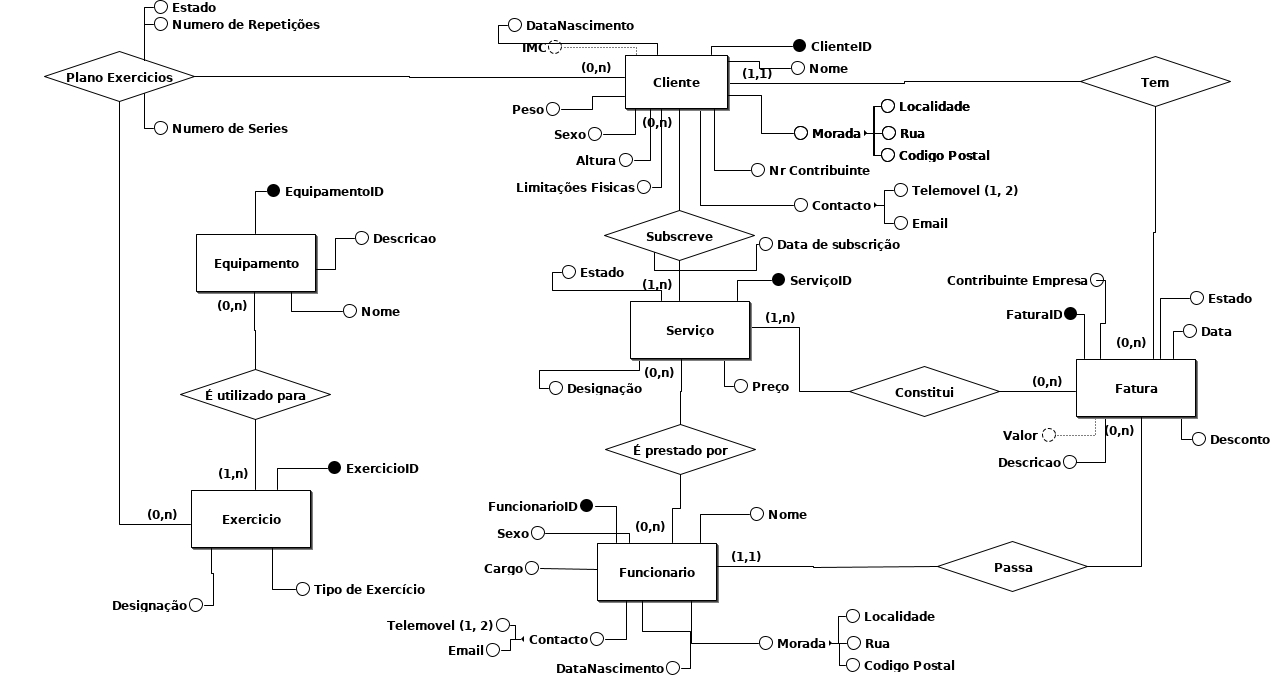
\includegraphics[width=\textwidth]{Conceptual/Conceptual10.png}
\caption{Modelo Conceptual.}
\label{fig:concetual}
\end{figure}

Como já foi dito anteriormente, com o intuito de modelar todas as entidades da nossa base de dados e os relacionamentos entre elas, criamos um diagrama ER usando notação \textbf{Peter Chen} por motivos de organização. Este diagrama é constituído pelas nossas sete entidades as quais estão ligadas entre si através dos relacionamentos já apresentados no grupo 3.3.\par
Uma das razões de se usar um diagrama deste tipo é que este permite-nos chegar a um entendimento mais preciso em relação ao que o senhor Miguel de facto quer / precisa. De facto, é mais fácil visualizar um diagrama de entidades e relacionamentos complexo, do que ler e entender um longo texto com todos os requerimentos do senhor Miguel. Isto acontece pois, por vezes podemos fazer interpretações erradas de alguns requerimentos ou até, o autor dos mesmos pode não os explicar de forma sucinta.\par
Assim, o uso de um diagrama ER permite-nos ter uma visualização do problema bastante mais simplificada e organizada proporcionando-nos uma valiosa ferramenta que será a base de todo este projeto. 

\section{Validação do modelo de dados com o utilizador}

A fim de finalizar todo este processo de modelação, foi necessário que o senhor Miguel o confirmasse e validasse.\par
No final da criação do modelo ER, juntamo-nos mais uma vez com o nosso cliente para, se necessário, retificar alguma gralha no modelo conceptual. 
Alteramos e corrigimos vários detalhes e anomalias referentes ao modelo até que o senhor Miguel ficasse satisfeito.\par
Foi nesta fase que, aquando da aprovação e validação do modelo conceptual como uma  verdadeira representação da realidade na qual o modelo incide (o ginásio), por parte do nosso cliente, este o assinou, marcando assim o fim desta etapa fazendo com que pudéssemos avançar para o modelo lógico.






\chapter{Modelação Lógica}

% tirar isto? ou é melhor deixar e tentar incorporar?
%\section{Construção e validação do modelo de dados lógico}

Nesta capítulo, traduzimos o modelo concetual (fig. \ref{fig:concetual}) num modelo de dados lógico adequado aos dados do ginásio. Para tal, seguimos o processo descrito em \cite{dbsys}.

\section{Derivar relações para o modelo de dados lógicos}

Começamos por derivar relações a partir do modelo concetual seguindo as regras adequadas, de modo a representar no modelo lógico as entidades, relacionamentos e atributos identificados previamente. Tal gerou as seguintes relações. No entanto, para as relações Cliente e Funcionário, decidimos separar os atributos compostos \emph{Contacto} e \emph{Morada} nas suas próprias relações, em vez de colocar os respetivos atributos atómicos nas relações mencionadas, de forma a facilitar a compreensão.


\noindent
\\\textbf{Cliente} (ClienteID,  Nome, DataNascimento, Sexo, Peso, Altura, IMC, Limitações Físicas,  NrContribuinte, idContacto, idMorada)
\\\textbf{Primary Key} ClienteID
\\\textbf{Foreign Key} idContacto \textbf{references} Contacto(idContacto)
\\\textbf{Foreign Key} idMorada \textbf{references} Morada(idMorada)

\noindent
\\\textbf{Contacto} (idContacto, Telemóvel 1, Telemóvel 2, Email)
\\\textbf{Primary Key} idContacto

\noindent
\\\textbf{Morada} (idMorada, Rua, Localidade, CodigoPostal)
\\\textbf{Primary Key} idMorada

\noindent
\\\textbf{Serviço} (ServiçoID, Designação, Preço, Estado)
\\\textbf{Primary Key} ServiçoID

\noindent
\\\textbf{Fatura} (FaturaID, Contribuinte Empresa, Data, Desconto, Descrição, Valor, ClienteID, FuncionárioID, Estado)
\\\textbf{Primary Key} FaturaID
\\\textbf{Foreign Key} ClienteID \textbf{references} Cliente(ClienteID)
\\\textbf{Foreign Key} FuncionárioID \textbf{references} Funcionário(FuncionárioID)

\noindent
\\\textbf{Funcionário} (FuncionárioID, Nome, Cargo, Idade, idContacto, idMorada)
\\\textbf{Primary Key} FuncionárioID
\\\textbf{Foreign Key} idContacto \textbf{references} ContactoFuncionario(idContacto)
\\\textbf{Foreign Key} idMorada \textbf{references} MoradaFuncionario(idMorada)

\noindent
\\\textbf{ContactoFuncionario} (idContacto, Telemóvel 1, Telemóvel 2, Email)
\\\textbf{Primary Key} idContacto

\noindent
\\\textbf{MoradaFuncionario} (idMorada, Rua, Localidade, CodigoPostal)
\\\textbf{Primary Key} idMorada

\noindent
\\\textbf{Exercício} (ExercícioID, Designação, Tipo de Exercício)
\\\textbf{Primary Key} ExercícioID

\noindent
\\\textbf{Equipamento} (EquipamentoID, Descrição, Nome)
\\\textbf{Primary Key} EquipamentoID

% *:* relationship
\noindent
\\\textbf{Constitui} (ServiçoID, FaturaID)
\\\textbf{Primary Key} ServiçoID, FaturaID
\\\textbf{Foreign Key} ServiçoID \textbf{references} Serviço(ServiçoID)
\\\textbf{Foreign Key} FaturaID \textbf{references} Fatura(FaturaID)

% *:* relationship
\noindent
\\\textbf{Subscreve} (ClienteID, ServiçoID, Data Subscrição)
\\\textbf{Primary Key} ClienteID, ServiçoID
\\\textbf{Foreign Key} ClienteID \textbf{references} Cliente(ClienteID)
\\\textbf{Foreign Key} ServiçoID \textbf{references} Serviço(ServiçoID) 

% *:* relationship
\noindent
\\\textbf{E prestado por} (ServiçoID, FuncionárioID, Data Início)
\\\textbf{Primary Key} ServiçoID, FuncionárioID
\\\textbf{Foreign Key} ServiçoID \textbf{references} Serviço(ServiçoID)
\\\textbf{Foreign Key} FuncionárioID \textbf{references} Funcionário(FuncionárioID)

% *:* relationship
\noindent
\\\textbf{Plano Exercícios} (ClienteID, ExercicioID, Numero de Repetições, Numero de Series)
\\\textbf{Primary Key} ClienteID, ExercicioID
\\\textbf{Foreign Key} ClienteID \textbf{references} Cliente(ClienteID)
\\\textbf{Foreign Key} ExercicioID \textbf{references} Exercício(ExercicioID)

% *:* relationship
\noindent
\\\textbf{É utilizado para} (EquipamentoID, ExercícioID)
\\\textbf{Primary Key} EquipamentoID, ExercícioID
\\\textbf{Foreign Key} EquipamentoID \textbf{references} Equipamento(EquipamentoID)
\\\textbf{Foreign Key} ExercícioID \textbf{references} Exercício(ExercícioID)



\section{Desenho do modelo lógico}

A conversão das relações derivadas anteriormente resultou no modelo lógico representado na figura \ref{fig:mod_logico}.

\begin{figure}[h]
\begin{center}
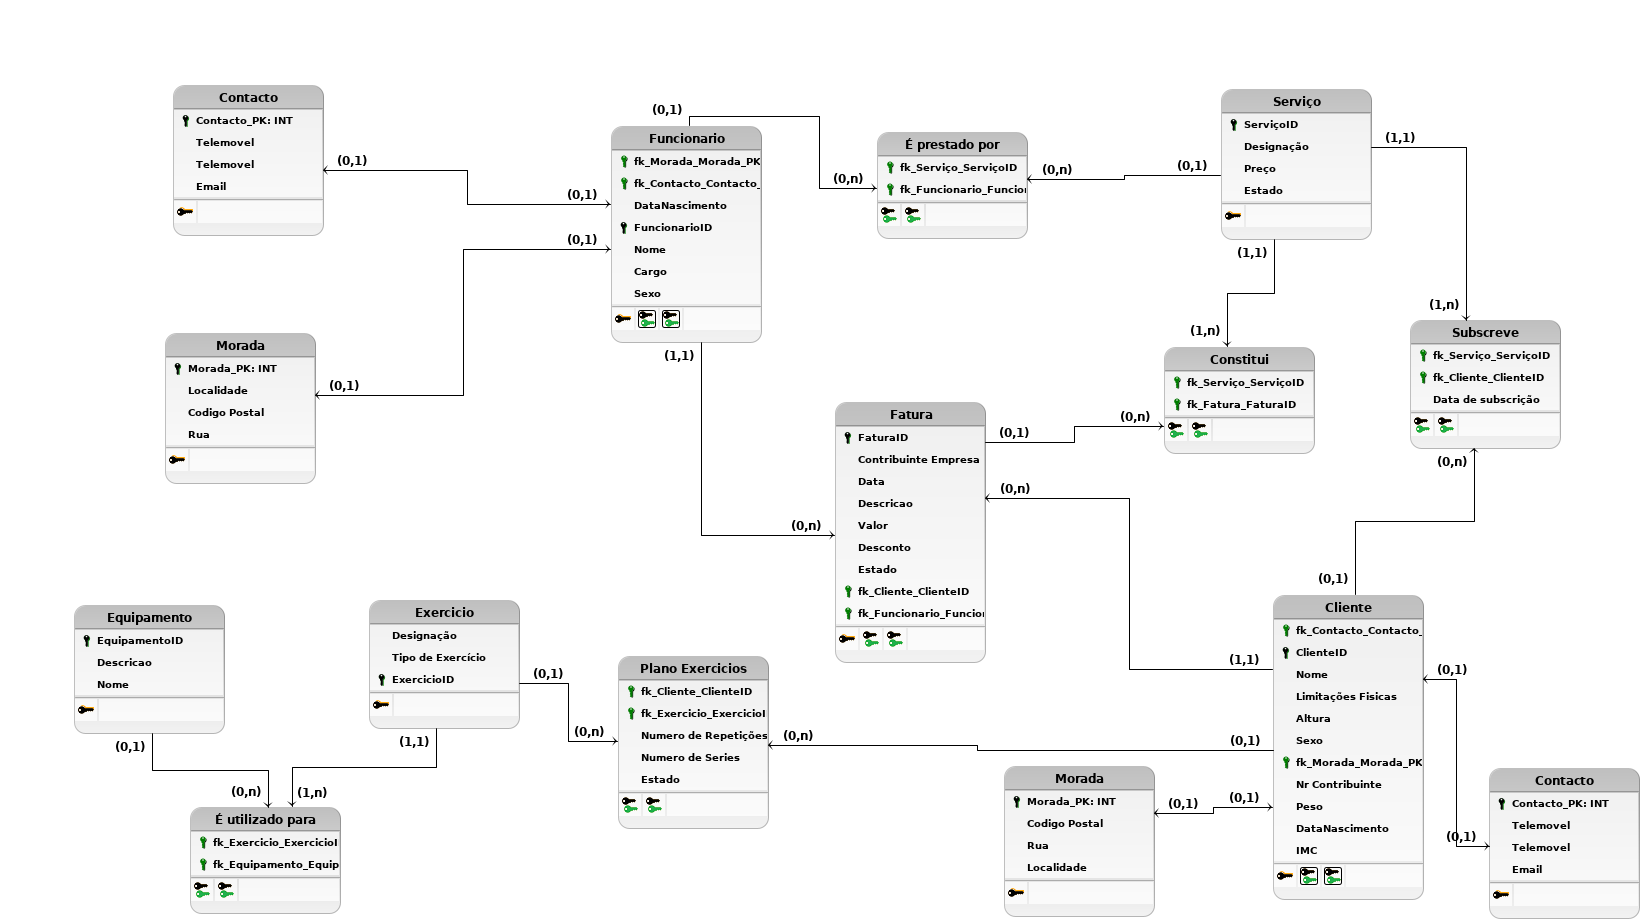
\includegraphics[width=\textwidth]{modelacao_logica/logicoBR.png}
\caption{Modelo Lógico}
\label{fig:mod_logico}
\end{center}
\end{figure}


\section{Validação do modelo através da normalização}

\subsection{Dependências Funcionais}

\noindent
\\\textbf{Cliente:}
\\ClienteID ®  Nome, Idade, Sexo, Peso, Altura, IMC, Limitações Físicas,  NrContribuinte, idContacto, idMorada
\\NrContribuinte ® ClienteID, Nome, Idade, Sexo, Peso, Altura, IMC, Limitações Físicas, idContacto, idMorada
\\idContacto ® ClienteID, Nome, Idade, Sexo, Peso, Altura, IMC, Limitações Físicas, NrContribuinte, idMorada

\noindent
\\\textbf{Contacto:}
\\idContacto ® Telemóvel 1, Telemóvel 2, Email

\noindent
\\\textbf{Morada:}
\\idMorada ® Rua, Localidade, CodigoPostal

\noindent
\\\textbf{Serviço:}
\\ServiçoID ® Designação, Preço

\noindent
\\\textbf{Fatura:}
\\FaturaID ® Contribuinte Empresa, Data, Desconto, Descrição, Valor, ClienteID, FuncionárioID

\noindent
\\\textbf{Funcionário:}
\\FuncionárioID ® Nome, Cargo, Idade, idContacto, idMorada

\noindent
\\\textbf{ContactoFuncionario:}
\\idContacto ® Telemóvel 1, Telemóvel 2, Email

\noindent
\\\textbf{MoradaFuncionario:}
\\idMorada ® Rua, Localidade, CodigoPostal

\noindent
\\\textbf{Exercício:}
\\ExercícioID ® Designação, Tipo de Exercício

\noindent
\\\textbf{Equipamento:}
\\EquipamentoID ® Descrição, Nome

\noindent
\\\textbf{Subscreve:}
\\ClienteID, ServiçoID ® Data Subscrição

\noindent
\\\textbf{E prestado por:}
\\ServiçoID, FuncionárioID ® Data Início

\noindent
\\\textbf{Plano Exercícios:}
\\ClienteID, ExercicioID ® Numero de Repetições, Numero de Series



\subsection{Primeira Forma Normal (1FN)}

Todas as relações estão na Primeira Forma Normal, pois, para cada relação, a interseção de uma linha e uma coluna contém apenas um valor.

\subsection{Segunda Forma Normal (2FN)}

As relações estão na Segunda Forma Normal, pois cada relação está na 1FN e todos os atributos não chave primária dessa relação dependem da totalidade da chave primária.

\subsection{Terceira Forma Normal (3FN)}

As relações estão na Terceira Forma Normal, pois cada relação está na 1FN e na 2FN e todos os atributos não chave primária dessa relação e dependem diretamente da chave primária, ou seja, não existem dependências transitivas.

\section{Validação do modelo com interrogações do utilizador}
\label{interrogacoes}

As seguintes interrogações proveem da secção \ref{subsec:requisitos}, composta por interrogações e transações. Iremos validar estas interrogações verificando que toda a informação necessária à sua realização (entidades, atributos e relacionamentos) está presente no modelo. As transações serão validadas na secção \ref{transacoes}.

\noindent
\\\textbf{Tem de ser possível visualizar que serviços são prestados por que funcionários.}
\\ As entidades Serviço e Funcionário, que compreendem os detalhes dos serviços e dos funcionários, respetivamente, estão representadas no modelo. Podemos usar o relacionamento \emph{Serviço É Prestado Por Funcionário} para extrair a informação requerida.

\noindent
\\\textbf{O responsável do ginásio poderá também consultar os serviços fornecidos pelo ginásio}
\\ $ \pi_{Designacao} (Servico) $

\noindent
\\\textbf{Para posterior confirmação dos updates ou adições referentes ao funcionário, o administrador deverá poder visualizar o conteúdo da tabela dos funcionários}
\\ $ \pi (Funcionario) $

\noindent
\\\textbf{Existe a necessidade de aceder à ficha do cliente pelo número de utilizador}
\\ A entidade Cliente representa os dados do cliente, que tem um número de utilizador único (o atributo ClienteID), logo a operação é possível.

\noindent
\\\textbf{Também deverá ser possível aceder à ficha do cliente através do seu número de telefone, caso este não saiba o seu idCliente}
\\ A entidade Cliente representa os dados do cliente e os contactos dos clientes estão representados na relação Contacto. A entidade Cliente tem como uma \emph{Foreign Key} o identificador do contacto do cliente na tabela Contacto, pelo que é possível associar a um cliente ao seu número de telefone e, assim, aceder aos dados do cliente a partir deste.

\noindent
\\\textbf{Terá de ser possível ao funcionário consultar os exercícios de um cliente}
\\ A entidade Cliente representa os dados do cliente e a entidade Exercício representa os exercícios no modelo lógico. Utilizando o relacionamento \emph{Plano Exercícios}, é possível consultar a informação requerida.

\noindent
\\\textbf{Deverá ser possível a consulta de todas as faturas emitidas pelo ginásio relativas a um cliente}
\\ As entidades Cliente e Fatura representam, respetivamente, os clientes (e os seus dados) e as faturas (e os seus dados). Utilizando o relacionamento \emph{Cliente Tem Fatura}, podemos produzir a lista de todas as faturas relatias a um cliente.

\noindent
\\\textbf{A consulta de faturas entre duas datas específicas será também uma funcionalidade presente na base de dados}
\\ A entidade Fatura, que representa as faturas no modelo lógico, tem um atributo NN \emph{Data}, que guarda a data de emissão da fatura, pelo que a operação é possível.

\noindent
\\\textbf{O responsável reserva-se o dever de ter acesso ao total faturado num determinado período de tempo ou durante todo o tempo de vida do ginásio}
\\ A entidade Fatura, que representa as faturas no modelo lógico, tem um atributo NN \emph{Data}, que guarda a data de emissão da fatura, e um atributo NN \emph{Valor}, que guarda o valor total da fatura, portanto, a interrogação é válida.

\noindent
\\\textbf{Quer o administrador quer os rececionistas devem poder ver que serviços foram registados em cada fatura}
\\ As entidades Serviço e Fatura representam, respetivamente, os serviços providenciados pelo ginásio e as faturas emitidas por este no modelo. Utilizando o relacionamento \emph{Serviço Constitui Fatura}, é possível visualizar a informação pretendida.

\noindent
\\\textbf{Os funcionários devem poder também ver quais as subscrições dos clientes}
\\  As entidades Cliente e Fatura representam, respetivamente, os clientes (e os seus dados) e os serviços do ginásio. Utilizando o relacionamento \emph{Cliente Subscreve Serviço}, é possível saber quais as subscrições dos clientes.


\section{Validação do modelo com as transações estabelecidas}
\label{transacoes}

As seguintes transações proveem da secção \ref{subsec:requisitos}, composta por interrogações e transações. Iremos validar estas transações verificando que toda a informação necessária à sua realização (entidades, atributos e relacionamentos) está presente no modelo. As interrogações foram validadas na secção \ref{interrogacoes}.


\noindent
\\\textbf{Terá de ser possível ao responsável do ginásio adicionar um funcionário}
\\ A entidade Funcionário, que representa os funcionários e os seus dados, existe no modelo, pelo que é possível adicionar funcionários à BD.

\noindent
\\\textbf{Terá também  de ser possível ao administrador do ginásio alterar a informação relativa a um funcionário}
\\ É possível, por consequência direta da existência da entidade Funcionário.

\noindent
\\\textbf{Outra das funções do administrador do ginásio será adicionar novos serviços que poderão vir a ser disponibilizados aos clientes}
\\ A entidade Serviços, que representa os serviços oferecidos pelo ginásio, existe, pelo que esta transação é válida.

\noindent
\\\textbf{Este terá também a obrigação de marcar como não disponíveis os serviços que entretanto forem descontinuados ou os quais o ginásio já não suporte}
\\  A entidade Serviços, que representa os serviços oferecidos pelo ginásio, existe, e contém o atributo Estado, que representa os serviços ativos ou descontinuados. Portanto, a transação é válida.

\noindent
\\\textbf{Terá de ser possível ao funcionário registar um novo cliente}
\\ A entidade Cliente, que representa os clientes e os seus dados, existe no modelo, pelo que é possível adicionar clientes à BD.

\noindent
\\\textbf{O funcionário deverá ter permissões para adicionar novos exercícios a um cliente}
\\ As entidades Cliente e Exercício representam, respetivamente, os clientes (e os seus dados) e os exercícios (e os seus dados) e estão ligadas pelo relacionamento binário \emph{Plano Exercícios}, pelo que é possível associar exercícios a um cliente.

\noindent
\\\textbf{Para além disso terá de ser também disponibilizada forma de apagar os exercícios associados a um cliente do seu plano de treinos}
\\ É possível, como consequência direta da transação anterior ser válida.

\noindent
\\\textbf{Ao funcionário reserva-se o dever de emitir faturas}
\\ No modelo existe a entidade Fatura, que representa as faturas emitidas pelo ginásio. Portanto, a emissão de faturas é possível.

\noindent
\\\textbf{Ao funcionário reserva-se também o dever de marcar uma fatura como inválida sempre que esta for mal inserida no sistema}
\\ A entidade Fatura tem o atributo Estado, que guarda se a fatura é válida ou não. Portanto, esta transação é válida.

\noindent
\\\textbf{Cabe ao funcionário designar qual o equipamento a ser utilizado num determinado exercício no momento da inserção deste na base de dados}
\\ As entidades Exercício e Equipamento, que representam os exercícios e os equipamentos disponibilizados pelo ginásio, existem no modelo. Utilizando o relacionamento \emph{Equipamento É Utilizado Para Exercício}, é possível associar equipamentos a exercícios. A transação é válida

\noindent
\\\textbf{No ginásio é requerida a necessidade de poder adicionar novos equipamentos}
\\ A transação é válida, pois a entidade Equipamento representa os equipamentos disponíveis no ginásio, pelo que é possível serem adicionados mais.

\noindent
\\\textbf{Um funcionário pode decidir adicionar um novo exercício aos atualmente disponíveis para os clientes}
\\ A transação é válida, pois a entidade Exercício representa os exercícios disponibilizados pelo ginásio, pelo que é possível serem adicionados mais.

\noindent
\\\textbf{O administrador será responsável por referenciar que funcionários executam que serviço}
\\ As entidades Funcionário e Serviço, que representam os funcionários do ginásio e os serviços oferecidos, existem no modelo, e, utilizando o relacionamento \emph{Serviço É Prestado Por Funcionário}, é possível associar um serviço a um funcionário, pelo que a transação é válida.


\section{Revisão do modelo lógico com o utilizador}

Após a finalização do modelo lógico, este foi apresentado ao cliente numa reunião, onde foi analisado em conjunto com este, para se determinar se o modelo realmente corresponde à realidade do ginásio. O cliente demonstrou-se bastante satisfeito com o resultado e este modelo lógico foi aprovado.
\chapter{Implementação Física}
\section{Seleção do sistema de gestão de bases de dados}
Optamos pela implementação duma base de dados usando o motor de base de dados MySQL.Trata-se dum motor de base de dados muito renomeado e quase padronizado pela industria, devido a sua elevada segurança dos dados, alto desempenho e pela sua capacidade de otimizar o programa reduzindo o tempo de execução. \par 
O MySQL ser um  motor de base de dados gratuito também contribuiu para a sua escolha, pois permite que seja possível a criação duma base de dados dentro dum orçamento mais amigável para o cliente.


\section{Tradução do esquema lógico para o sistema de gestão de bases de dados escolhido em SQL}

\begin{figure}[h]
\centering
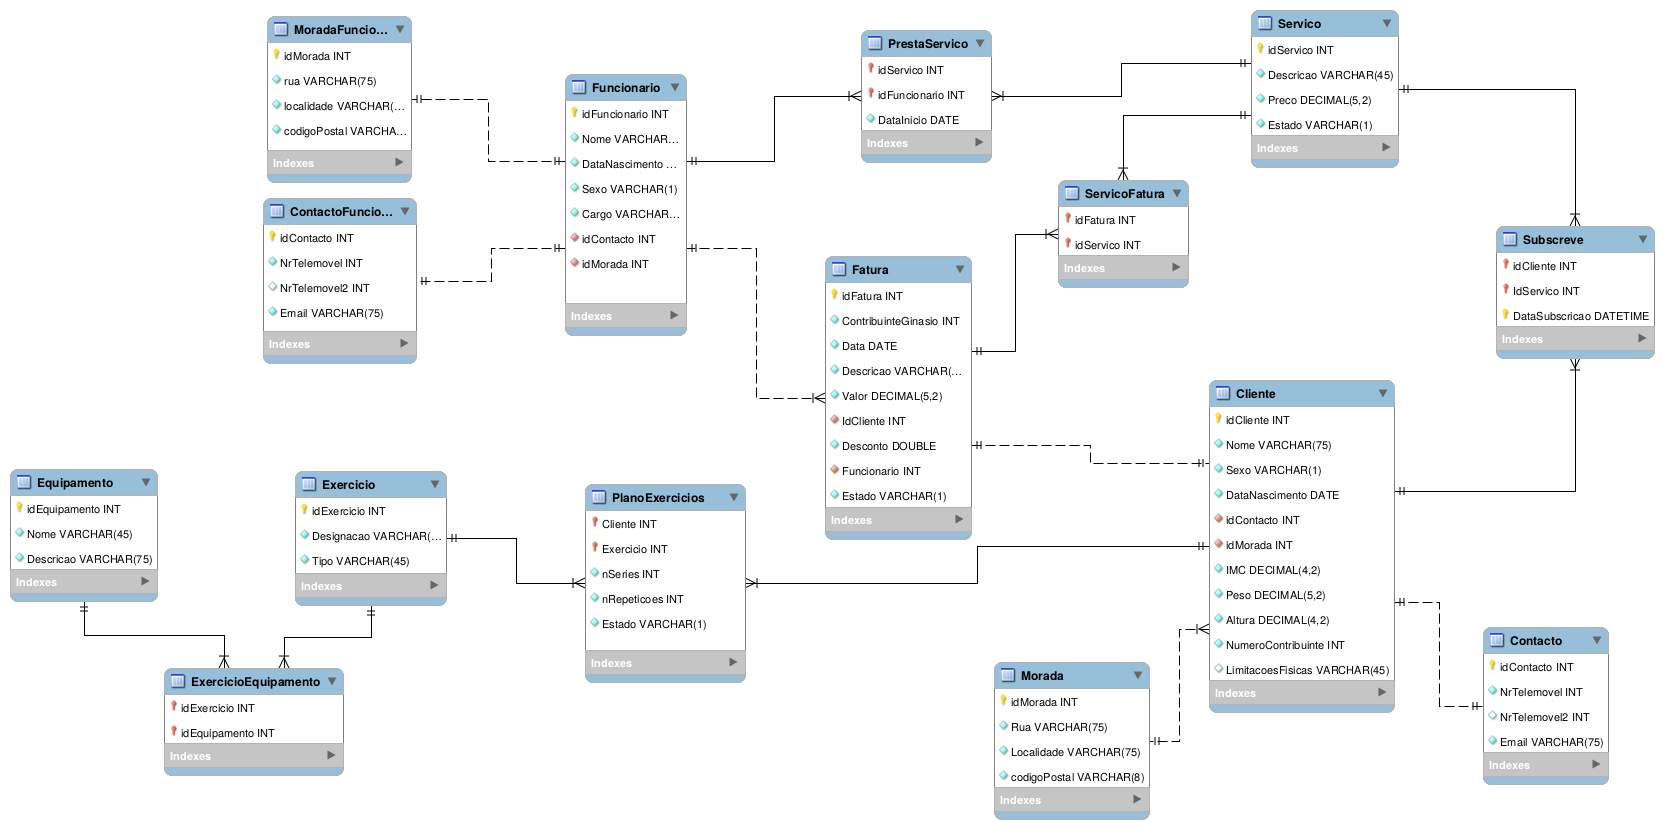
\includegraphics[width=\textwidth]{implementacao_fisica/ModeloLogico.png}
\caption{Modelo Lógico representado no MySQL Workbench}
\label{fig:mod_logico_mysql}
\end{figure}

\clearpage

\section{Tradução das interrogações do utilizador para SQL (alguns exemplos)}

\subsection{Interrogação faturação num mês}
\begin{lstlisting}[language=SQL]
    SELECT SUM(Valor) FROM Fatura as F
	    WHERE MONTH(F.Data)=01 AND YEAR(F.DATA)=2018; 
\end{lstlisting}

\begin{figure}[h]
\begin{center}
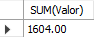
\includegraphics[scale=0.7]{implementacao_fisica/soma.png}
\centering
\end{center}
\end{figure}

\subsection{Todos os clientes que fizeram 'Martelo'}
\begin{lstlisting}[language=SQL]
SELECT IdCliente, Nome  FROM Cliente as C
	INNER JOIN planoexercicios as P on P.Cliente=C.idCliente
	INNER JOIN exercicio as E on P.Exercicio=E.idExercicio
	WHERE E.Designacao='Martelo';
\end{lstlisting}

\begin{figure}[h]
\begin{center}
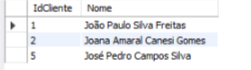
\includegraphics[scale=1.0]{implementacao_fisica/ClientesMartelo.png} 
\centering
\end{center}
\end{figure}

\subsection{A que serviços o cliente 1 está subscrito}
\begin{lstlisting}[language=SQL]
SELECT Descricao,nome  FROM Cliente as C
	INNER JOIN subscreve as S on C.idCliente=S.idCliente
    INNER JOIN servico as Z on S.Idservico=Z.idservico
    WHERE (C.idCliente=1);
\end{lstlisting}

\begin{figure}[h]
\begin{center}
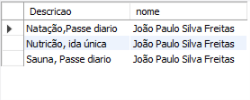
\includegraphics[scale=1.0]{implementacao_fisica/Servicoscliente1.png} 
\centering
\end{center}
\end{figure}

\subsection{Faturas correspondentes ao cliente 2}
\begin{lstlisting}[language=SQL]
SELECT idFatura,Valor FROM fatura as F
	INNER JOIN Cliente as C on F.idCliente=C.idCliente
    WHERE C.idCliente=2;
    
\end{lstlisting}
\begin{figure}[h]
\begin{center}
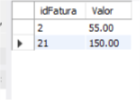
\includegraphics[scale=1.0]{implementacao_fisica/Desenho.png} 
\centering
\end{center}
\end{figure}

\section{Tradução das transações estabelecidas para SQL (alguns exemplos)}
Quando um cliente é criado, também é criado a morada e o seu contacto, usando as transações os contactos e a morada só são criados se e só se o cliente também for criado.
\begin{lstlisting}[language=SQL]

CREATE DEFINER=`root`@`localhost` PROCEDURE `Nova Ficha de Cliente`(in nome VARCHAR(75),in idade INT,in sexo VARCHAR(1),in peso INT, in altura INT,in numerocontribuinte INT, in limitacoesfisicas VARCHAR(75),in telemovel1 INT, in telemovel2 INT ,email VARCHAR(75),rua VARCHAR(75),localidade VARCHAR(75),codigopostal VARCHAR(75))
BEGIN
DECLARE x INT;
DECLARE y INT;
DECLARE z INT;
 DECLARE EXIT HANDLER FOR SQLEXCEPTION
   BEGIN
      ROLLBACK;
      RESIGNAL;
   END;

START TRANSACTION;


 SET z = peso /POWER(altura,2);
INSERT INTO morada
	(Rua,Localidade,codigoPostal)
    VALUES
		(rua,localidade,codigopostal);
 SET x=  LAST_INSERT_ID();
        
INSERT INTO contacto
		(NrTelemovel,NrTelemovel2,Email)
        Values
			(telemovel1,telemovel2,email);
SET y=LAST_INSERT_ID();
INSERT INTO cliente
	(Nome,Sexo,Idade,idContacto,IdMorada,IMC,Peso,Altura,NumeroContribuinte,LimitacoesFisicas)
    Values
		(nome,sexo,idade,x,y,z,peso,altura,numerocontribuinte,limitacoesfisicas);
        COMMIT;
 END
\end{lstlisting}
\clearpage
Tal como nos clientes, nos apenas podemos adicionar o contacto e a morada do funcionario se a adição do funcionario também foi um sucesso
\begin{lstlisting}[language=SQL]
CREATE DEFINER=`root`@`localhost` PROCEDURE `Criacao da Ficha de novo Funcionario`(in nome VARCHAR(75),in idade INT,in sexo VARCHAR(1),in cargo VARCHAR(75),in telemovel1 INT, in telemovel2 INT ,email VARCHAR(75),rua VARCHAR(75),localidade VARCHAR(75),codigopostal VARCHAR(75))
BEGIN
DECLARE x INT;
DECLARE y INT;
DECLARE EXIT HANDLER FOR SQLEXCEPTION
   BEGIN
      ROLLBACK;
      RESIGNAL;
   END;
   START TRANSACTION;
INSERT INTO moradafuncionario
	(Rua,Localidade,codigoPostal)
    VALUES
		(rua,localidade,codigopostal);

SET x=  LAST_INSERT_ID();
        
INSERT INTO contactofuncionario
		(NrTelemovel,NrTelemovel2,Email)
        Values
			(telemovel1,telemovel2,email);
SET y=LAST_INSERT_ID();
INSERT INTO funcionario
	(Nome,Idade,Sexo,Cargo,idContacto,IdMorada)
    Values
		(nome,idade,sexo,cargo,y,x);
COMMIT;
END
\end{lstlisting}

\section{Escolha, definição e caracterização de índices em SQL (alguns exemplos)}
Implementamos um índice no nosso Plano de Exercícios uma vez que é uma tabela que ao longo do tempo vai ficar extremamente populada, pois para cada cliente vamos preencher vários exercícios, como tal para encontrar o plano de exercícios dum cliente criamos um índice na coluna do idCliente para facilitar a sua procura.
\par Pensamos ainda implementar um índice na tabela dos clientes, mas como ainda se trata dum pequeno ginásio, a expectativa de número de clientes não justifica a implementação dum índice. 

\clearpage
\section{Estimativa do espaço em disco da base de dados e taxa de crescimento anual}
Para a estrutura de base de dados no seu estado atual e considerando os tamanhos máximos permitidos nas várias estruturas, temos uma ocupação máxima  de espaço dividida para cada elemento inserido.

\vspace{15pt}
\noindent
\textbf{Exemplo de cálculo do espaço ocupado:}

\begin{table}[h]
\resizebox{\textwidth}{!}{
\begin{tabular}{|l|c|}
\hline
\multicolumn{1}{|c|}{\textbf{Espaço ocupado pela tabela Cliente}}                                                                                                                                                                                               & \multicolumn{1}{l|}{\textbf{Total em Bytes}} \\ \hline
Primeiro de tudo, o Cabeçalho, ocupa 4 bytes.                                                                                                                                                                                        & 4 bytes                                      \\ \hline
Data Type que tem valor fixo(INT)5x4                                                                                                                                                                                                 & 20 bytes                                     \\ \hline
Null Block = 2 bytes, pois temos 11 campos                                                                                                                                                                                           & 2 bytes                                      \\ \hline
Variable Block = 2 bytes + 12bytes (2 para cada campo com dados variáveis, nos temos 6)                                                                                                                                              & 14 bytes                                     \\ \hline
\begin{tabular}[c]{@{}l@{}}Data Types com valores variáveis (nome varchar(75),sexo varchar(1),IMC decimal(4,2), \\                              Peso decimal(5,2), altura(decimal(4,2) e limitações físicas varchar(45)\end{tabular} & 134 bytes                                    \\ \hline
\textbf{Total}                                                                                                                                                                                                                       & 174 bytes                                    \\ \hline
\end{tabular}
}
\end{table}
\begin{itemize}
\item Um cliente ocupa 174bytes+96bytes do contacto +  175bytes da morada,ou seja, 445 bytes
\item Um funcionário ocupa 154 bytes +96bytes para contacto + 175 bytes para a morada,ou seja,425 bytes
\item Uma fatura ocupa 149 bytes
\item Um serviço ocupa 68 bytes
\item Um exercício ocupa 135 bytes
\item Um equipamento ocupa 138 bytes
\item Uma relação entre serviço e funcionário ocupa 15 bytes
\item Uma relação entre serviço e cliente ocupa  23 bytes
\item Uma relação entre serviço e fatura ocupa 15 bytes
\item Uma relação entre cliente e exercício ocupa 23 bytes
\item Uma relação entre exercício e equipamento ocupo 15 bytes

Tendo em conta que a base de dados no estado atual tem 20 clientes, 8 funcionários,9 serviços, 18 equipamentos, 22 exercícios, 82 exercícios dedicados aos clientes ,6 serviços a ser prestados aos clientes pelos funcionários, existem 35 inscrições dos clientes nos serviços,20 serviços faturados,23 exercícios utilizam equipamento e 20 faturas, temos :

\begin{lstlisting}[literate=%
        {é}{{\'{e}}}1
        {è}{{\`{e}}}1
        {ê}{{\^{e}}}1
        {ë}{{\¨{e}}}1
        {É}{{\'{E}}}1
        {Ê}{{\^{E}}}1
        {û}{{\^{u}}}1
        {ù}{{\`{u}}}1
        {ú}{{\'{u}}}1
        {â}{{\^{a}}}1
        {à}{{\`{a}}}1
        {á}{{\'{a}}}1
        {ã}{{\~{a}}}1
        {Á}{{\'{A}}}1
        {Â}{{\^{A}}}1
        {Ã}{{\~{A}}}1
        {ç}{{\c{c}}}1
        {Ç}{{\c{C}}}1
        {õ}{{\~{o}}}1
        {ó}{{\'{o}}}1
        {ô}{{\^{o}}}1
        {Õ}{{\~{O}}}1
        {Ó}{{\'{O}}}1
        {Ô}{{\^{O}}}1
        {î}{{\^{i}}}1
        {Î}{{\^{I}}}1
        {í}{{\'{i}}}1
        {Í}{{\~{Í}}}1]

20 x 445= 8900 B -> Clientes

8 x 425 = 3400 B -> Funcionário
9 x 68 = 612 B -> Serviço
18 x 138 = 2484 B -> Equipamento 
22 x 135 = 2970 B -> Exercícios
82 x 23 =1886 B -> Relacionamento exercício-cliente
6 x 15 =90 B -> Relacionamento serviço-funcionário
35 x 23 =805 B -> Relacionamento serviço-cliente
20 x 15 =300 B -> Relacionamento serviço-fatura
23 x 15 =345 B -> Relacionamento exercício-equipamento
20 x 149 = 2980 B -> Faturas

Total: 24 772 b = 24.19141 kB
\end{lstlisting}


Logo, a base de dados no estado atual tem aproximadamente 24.2kB ocupados.
\clearpage
O Sr. Miguel espera no próximo ano ter mais uma centena de clientes,subscrevendo se no mínimo a 1 serviço, cada um com pelo menos 5 exercícios( no intuito de balancear com os que se inscrevem apenas em nutrição,logo não tem exercícios), e para satisfazer as necessidades dos mesmos ele quer acrescentar 20 novos equipamentos e recrutar 5 novos funcionários, alem disso, planeia ter 2000 faturas ao final do ano.

\begin{lstlisting}[literate=%
        {é}{{\'{e}}}1
        {è}{{\`{e}}}1
        {ê}{{\^{e}}}1
        {ë}{{\¨{e}}}1
        {É}{{\'{E}}}1
        {Ê}{{\^{E}}}1
        {û}{{\^{u}}}1
        {ù}{{\`{u}}}1
        {ú}{{\'{u}}}1
        {â}{{\^{a}}}1
        {à}{{\`{a}}}1
        {á}{{\'{a}}}1
        {ã}{{\~{a}}}1
        {Á}{{\'{A}}}1
        {Â}{{\^{A}}}1
        {Ã}{{\~{A}}}1
        {ç}{{\c{c}}}1
        {Ç}{{\c{C}}}1
        {õ}{{\~{o}}}1
        {ó}{{\'{o}}}1
        {ô}{{\^{o}}}1
        {Õ}{{\~{O}}}1
        {Ó}{{\'{O}}}1
        {Ô}{{\^{O}}}1
        {î}{{\^{i}}}1
        {Î}{{\^{I}}}1
        {í}{{\'{i}}}1
        {Í}{{\~{Í}}}1]
        
100 x 445 = 44500 B-> Clientes
5 x 425 = 2125 B-> Funcionários
20 x 138 = 2760 B-> Equipamento
2000 x 149 = 298000 B-> Fatura
100 x 805 =  80500 B-> Relacionamento serviço-cliente
5 x 100 x 23 = 11500 B -> Relacionamento cliente-exercício
Total = 450885 B = 440.32 kB
\end{lstlisting}
\par Com base nestes dados no próximo ano a base de dados ocupará  24.1 + 440.32 =463.33 kB



\end{itemize}

\section{Definição e caracterização das vistas de utilização em SQL (alguns exemplos)}
Código da implementação da view que lista todos os clientes do Ginásio
\begin{lstlisting}[language=SQL]
CREATE VIEW `view_cliente` AS
    SELECT 
        C.idCliente,
        C.Nome,
        C.Sexo,
        C.Idade,
        C.IMC,
        C.Peso,
        C.Altura,
        C.NumeroContribuinte,
        C.LimitacoesFisicas,
        CC.NrTelemovel,
        CC.NrTelemovel2,
        CC.Email,
        M.Rua,
        M.Localidade,
        M.CodigoPostal
    FROM
        Cliente AS C
            INNER JOIN
        Contacto AS CC ON CC.idContacto = C.idContacto
            INNER JOIN
        Morada AS M ON M.idMorada = C.idMorada;
\end{lstlisting}

\begin{figure}[h]
\begin{center}
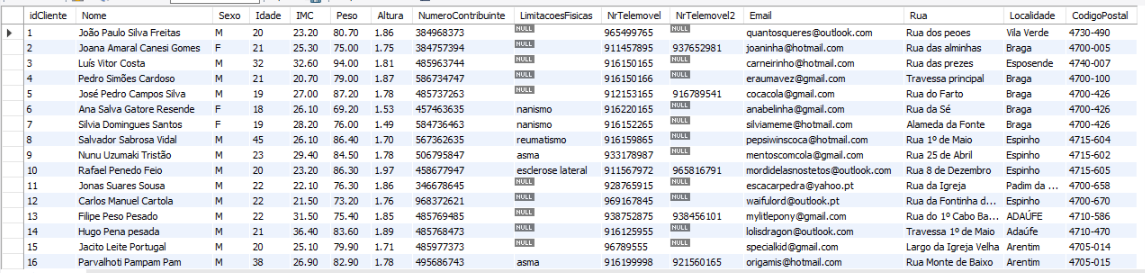
\includegraphics[scale=0.5]{implementacao_fisica/ViewCliente.png}
\centering
\end{center}
\end{figure}

\clearpage
Código da implementação da view que mostra todos os planos de exercícios.
\begin{lstlisting}[language=SQL]
CREATE VIEW `view_exerciciosCliente` AS

SELECT C.Nome AS NomeCliente, E.Designacao AS NomeExercicio, PE.nSeries,PE.nRepeticoes FROM PlanoExercicios AS PE
   INNER JOIN Exercicio AS E ON E.idExercicio = PE.Exercicio
   INNER JOIN Cliente AS C ON C.idCLiente = PE.Cliente;
\end{lstlisting}

\begin{figure}[h]
\begin{center}
%\includegraphics[scale=1.0]{implementacao_fisica/
\centering
\end{center}
\end{figure}
Código da implementação da view que mostra Os serviço(serviços que o cliente subscreveu) que cada funcionário faz
\begin{lstlisting}[language=SQL]
CREATE 
    ALGORITHM = UNDEFINED 
    DEFINER = `root`@`localhost` 
    SQL SECURITY DEFINER
VIEW `view_prestaservico` AS
    SELECT 
        `S`.`Descricao` AS `Descricao`,
        `F`.`Nome` AS `Nome`,
        `F`.`Cargo` AS `Cargo`,
        `S`.`Preco` AS `Preco`
    FROM
        ((`prestaservico` `PS`
        JOIN `servico` `S` ON ((`S`.`idServico` = `PS`.`idServico`)))
        JOIN `funcionario` `F` ON ((`F`.`idFuncionario` = `PS`.`idFuncionario`)))
    ORDER BY `S`.`Descricao`
\end{lstlisting}

\begin{figure}[h]
\begin{center}
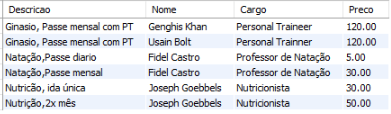
\includegraphics[scale=1.0]{implementacao_fisica/Prestaservico.png}
\centering
\end{center}
\end{figure}
\clearpage
Código da implementação da view que mostra a que serviços os clientes estão subscritos.
\begin{lstlisting}[language=SQL]
CREATE VIEW `view_subscricao` AS

SELECT C.Nome AS  NomeCliente, S.Descricao AS Servico, SUB.DataSubscricao FROM Subscreve AS SUB
   INNER JOIN Servico AS S ON S.idServico = SUB.idServico
   INNER JOIN Cliente AS C ON C.idCliente = SUB.idCliente;
\end{lstlisting}
\begin{figure}[h]
\begin{center}
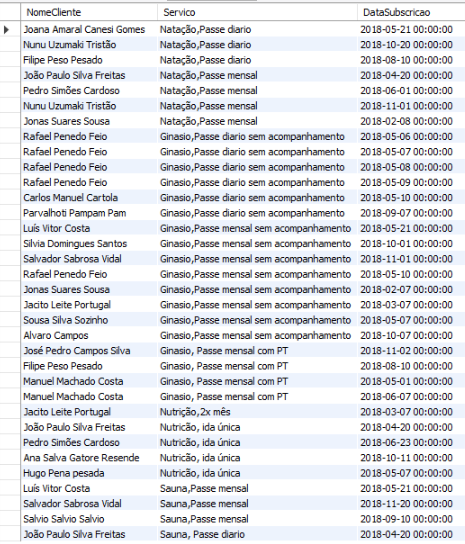
\includegraphics[scale=1.0]{implementacao_fisica/Susbricao.png}
\centering
\end{center}
\end{figure}
\clearpage
\section{Definição e caracterização dos mecanismos de segurança em SQL (alguns exemplos)}
Foram criados 2 users, um para cada rececionista , com apenas permissões de adicionar e dar update as linhas das tabelas, tenho como segurança que nenhum destes destroi uma tabela sem querer.
\begin{lstlisting}[language=SQL]
CREATE USER 'Jafar Strogonof'@'localhost' IDENTIFIED BY 'Jafar';

CREATE USER 'King Julian Move-it Move-it'@'localhost' IDENTIFIED BY 'Julian';

GRANT INSERT,UPDATE,EXECUTE, SHOW VIEW ON Ginasio.* TO 'Jafar Strogonof'@'localhost';
GRANT INSERT,UPDATE,EXECUTE, SHOW VIEW ON Ginasio.* TO 'King Julian Move-it Move-it'@'localhost';
\end{lstlisting}

\begin{figure}[h]
\begin{center}
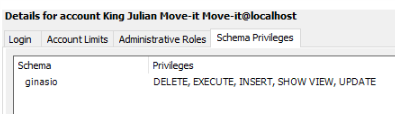
\includegraphics[scale=1.0]{implementacao_fisica/Previlegios.png}
\centering
\end{center}
\end{figure}
\par Sendo assim, o Sr. Miguel é a única pessoa com acesso administrativo a base de dados.

\section{Revisão do sistema implementado com o utilizador}
Após a implementação do sistema de base de dados, foi realizada uma reunião com o Sr.Miguel para ver se o produto final lhe agradava e receber algum feedback caso não estivesse do seu agrado.
\par Primeiramente o Sr.Miguel disse que não estávamos a cumprir completamente o seu pedido, ou seja, não tínhamos todos os procedimentos que este desejava, como por exemplo, adicionar um funcionário e um equipamento. Alargou-nos o prazo de entrega para a semana seguinte com o objetivo de  adicionarmos essas funções e para dar mais uns retoques onde fosse necessário.
\par Posteriormente, após a instalação e demonstração da execução destes novos procedimentos, o  Sr.Miguel ficou bastante satisfeito com o sistema de Base de Dados.
\chapter{Conclusões e Trabalho Futuro}

Neste trabalho construimos uma  base de dados para o ginásio do Sr. Miguel, cumprindo todos os requisitos que o mesmo nos  apresentou. De referir, que este trabalho se tornou mais extenso e trabalhoso do que o expectado, todavia o resultado final compensou a nossa dedicação uma vez que conseguimos alcançar a satisfação do nosso cliente e das metas que nos foram  colocadas. Gostaríamos de realçar ainda que este trabalho contribuiu para que fossemos capaz de desenvolver uma melhor capacidade de trabalho em equipa e de delegação de tarefas.  \par
Durante o desenvolvimento deste projeto, percebemos que o auxilio do motor de base de dados MySQL foi de grande importância visto que nos proporcionou ferramentas fundamentais para facilitar várias das nossas tarefas e garantir toda a consistência dos nossos dados.

\par O nosso maior desafio, mas também uma conquista foi conseguir chegar a um consenso no nosso modelo conceptual. Numa primeira etapa do desenvolvimento do projeto, o modelo parecia-nos correto, contudo tal não se verificou o que nos levou a investir uma grande quantidade de tempo a remodelar o mesmo para que tudo estivesse de acordo com o que o nosso cliente desejava e de acordo com as regras de normalização e das etapas da modelação lógica.\par
Para além disso, é de salientar que todo o processo de modelação, desde modelo conceptual até ao físico, é imprescindível na criação de uma base de dados para promover a organização e consistência de todo o processo. De facto, este método contribuiu imenso para o nosso sucesso.
\par Numa perspetiva futura, temos como objetivo implementar uma entidade Fornecedor que estaria encarregue da distribuição dos equipamentos e no caso de um equipamento avariar seria possível chegar ao fornecedor do mesmo e comunicar a necessidade da reparação do equipamento. Além disso queremos expandir a base de dados para mais ginásios, ou seja, criar uma entidade ginásio, permitindo nos comercializar facilmente a base de dados.


\part{Projeto de um Sistema de Bases de Dados não Relacional}
\chapter{Utilização de um sistema NoSQL}

Existem grandes vantagens em optar por um sistema não relacional (como o MongoDB) em vez de uma base de dados relacional:

\begin{itemize}
    \item  Consultas muito simples, mais fáceis de escrever, mais rápidas a executar e mais fáceis de ajustar às necessidades do inquiridor.

    \item Escalabilidade: um sistema SQL tem grandes problemas de escalabilidade.

    \item É suscetível a alterações conforme o desenvolvimento do ginásio, permitindo facilmente alterar e adicionar novas entidades e atributos ao esquema.

    \item Sharding: Sharding é um conceito simples: se tivermos uma quantidade enorme de dados de tal forma que o disco esteja praticamente cheio, a resposta é ter esse mesmos dados divididos entre várias máquinas. Para além de obtermos maior capacidade de armazenamento, também adquirimos maior rendimento. Como com o passar do tempo tanto a capacidade como a rapidez das bases de dados precisa de aumentar, basta aumentar o número de shards.

    \item GridFS: Normalmente quando queremos guardar uma foto numa base de dados guardamos o caminho para chegar a esta na nossa máquina.
    Com o GridFS podemos facilmente guardar arquivos desses na base de dados. O MongoDB foi construido tendo isso em conta, permitindo replicação e sharding desses mesmos arquivos, fornecendo a "backbone" de um sistema de arquivos partilhados.

\end{itemize}

No entanto, para o caso do ginásio, a utilização de um sistema NoSQL \textbf{não se justifica}, porque:
\begin{itemize}
    \item a base de dados é para um pequeno ginásio local. Como tal, este vai conter pequena quantidade de dados, não criando qualquer problema de escalabilidade num sistema SQL;
    \item trata-se de um modelo lógico bastante simples e estruturado;
    \item a base de dados estará sujeita a muitas operações de escrita. Devido à natureza desnormalizada de um sistema não relacional, tal teria um impacto negativo no desempenho da BD.
\end{itemize}

No entanto, no âmbito da disciplina, criaremos um sistema NoSQL de consulta utilizando o MongoDB. O sistema armazenará os dados necessários à execução de todas as queries, tendo um esquema otimizado para uma velocidade superior de execução de queries, quando comparado ao sistema relacional. Para tal, as escritas na BD serão feitas no sistema relacional, a partir do qual, após uma quantidade arbitrária de tempo, um programa atualizará o sistema NoSQL, que poderá receber e satisfazer queries.

\chapter{Modelação do sistema para uma \emph{Document Store}}

Como afirmado anteriormente, decidimos modelar esta BD não relacional para priorizar o desempenho da execução de queries. Para tal, desnormalizamos a BD, organizando a informação de modo a que toda a informação necessária para a realização de uma query esteja na mesma \emph{collection}.

Decidimos criar quatro \emph{collections}:
\begin{itemize}
    \item cliente
    \item fatura
    \item funcionario
    \item servico
\end{itemize}

Para cada coleção, armazenamos os seguintes atributos (ver tabela \ref{tab:noSQLatributos}):

\begin{table}[h]
\centering
\begin{tabular}{cl|c|l|}
\hline
\multicolumn{1}{|c|}{\multirow{14}{*}{\textbf{cliente}}} & id                 & \multirow{8}{*}{\textbf{funcionario}} & id                   \\
\multicolumn{1}{|c|}{}                                   & nome               &                                       & nome                 \\
\multicolumn{1}{|c|}{}                                   & sexo               &                                       & sexo                 \\
\multicolumn{1}{|c|}{}                                   & data de nascimento &                                       & data de nascimento   \\
\multicolumn{1}{|c|}{}                                   & imc                &                                       & cargo                \\
\multicolumn{1}{|c|}{}                                   & peso               &                                       & morada               \\
\multicolumn{1}{|c|}{}                                   & altura             &                                       & contacto             \\
\multicolumn{1}{|c|}{}                                   & contribuinte       &                                       & servicos             \\ \cline{3-4} 
\multicolumn{1}{|c|}{}                                   & limitacao          & \multirow{11}{*}{\textbf{fatura}}     & id                   \\
\multicolumn{1}{|c|}{}                                   & morada             &                                       & contribuinteGinasio  \\
\multicolumn{1}{|c|}{}                                   & contacto           &                                       & nomeFuncionario      \\
\multicolumn{1}{|c|}{}                                   & servicos           &                                       & nomeCliente          \\
\multicolumn{1}{|c|}{}                                   & exercicios         &                                       & NContribuinteCliente \\
\multicolumn{1}{|c|}{}                                   & faturas            &                                       & data                 \\ \cline{1-2}
\multicolumn{1}{|c|}{\multirow{4}{*}{\textbf{servico}}}  & id                 &                                       & descricao            \\
\multicolumn{1}{|c|}{}                                   & nome               &                                       & valor                \\
\multicolumn{1}{|c|}{}                                   & preco              &                                       & desconto             \\
\multicolumn{1}{|c|}{}                                   & estado             &                                       & funcionarioId        \\ \cline{1-2}
\multicolumn{1}{l}{}                                     &                    &                                       & estado               \\ \cline{3-4} 
\end{tabular}
\caption{Atributos armazenados para cada coleção}
\label{tab:noSQLatributos}
\end{table}

Após a migração (abordada no capítulo \ref{chapter:migracao}), esta modelação resulta em documentos como os exemplos que podem ser observados nas \emph{listings} \ref{json:clientes}, \ref{json:faturas}, \ref{json:funcionarios} e \ref{json:servicos}

%Clientes
\begin{lstlisting}[caption={Exemplo de documento: cliente},label={json:clientes}]
{
    "_id" : ObjectId("5c3e4621ada3f40448da749a"),
    "id" : 1,
    "nome" : "João Paulo Silva Freitas",
    "sexo" : "M",
    "dataNascimento" : "1998-10-10",
    "imc" : 23.2,
    "peso" : 80.7,
    "altura" : 1.86,
    "contribuinte" : 384968373,
    "limitcao" : null,
    "morada" : {
        "rua" : "Rua dos peoes",
        "localidade" : "Vila Verde",
        "codigoPostal" : "4730-490"
    },
    "contacto" : {
        "tele1" : 965499765,
        "tele2" : 0,
        "email" : "quantosqueres@outlook.com"
    },
    "servicos" : [ 
        {
            "id" : 2,
            "nome" : "Natação,Passe mensal",
            "data" : "2018-04-20 00:00:00",
            "preco" : 30.0
        }, 
        {
            "id" : 9,
            "nome" : "Sauna, Passe diario",
            "data" : "2018-04-20 00:00:00",
            "preco" : 3.0
        }
    ],
    "exercicios" : [ 
        {
            "id" : 1,
            "descricao" : "Agachamentos",
            "tipo" : "Pernas",
            "sets" : 4,
            "reps" : 10,
            "estado" : "A"
        }, 
        {
            "id" : 5,
            "descricao" : "Curl Invertido",
            "tipo" : "Bícep",
            "sets" : 4,
            "reps" : 10,
            "estado" : "A"
        },
        {
            "id" : 20,
            "descricao" : "Elevações Frontais Halteres",
            "tipo" : "Ombros",
            "sets" : 4,
            "reps" : 10,
            "estado" : "A"
        }
    ],
    "faturas" : [ 
        {
            "id" : 1,
            "contribuinteGinasio" : 111111111,
            "data" : "2018-01-05",
            "descricao" : "Natação, Mensal & Ginásio, Mensal, PersonalTrainer",
            "valor" : 150.0,
            "desconto" : 30.0,
            "funcionarioId" : 7,
            "invalida" : "A"
        }
    ]
}
\end{lstlisting}

%Faturas
\begin{lstlisting}[caption={Exemplo de documento: fatura},label={json:faturas}]
{
    "_id" : ObjectId("5c3e649045eb9b1e442bb13c"),
    "id" : 1,
    "contribuinteGinasio" : 111111111,
    "nomeFuncionario" : "Jafar Strogonof",
    "nomeCliente" : "João Paulo Silva Freitas",
    "NContribuinteCliente" : 384968373,
    "data" : "2018-01-05",
    "descricao" : "Natação, Mensal & Ginásio, Mensal, PersonalTrainer",
    "valor" : 150.0,
    "desconto" : 30.0,
    "funcionarioId" : 7,
    "estado" : "A"
}
\end{lstlisting}

%Funcionarios
\begin{lstlisting}[caption={Exemplo de documento: funcionario},label={json:funcionarios}]
{
    "_id" : ObjectId("5c3e4621ada3f40448da74c2"),
    "id" : 1,
    "nome" : "Josef Stalini",
    "data" : "1990-12-10",
    "sexo" : "M",
    "cargo" : "Empregado de Limpeza",
    "morada" : {
        "rua" : "Rua de Pousada",
        "localidade" : "Gualtar",
        "codigoPostal" : "4710-049"
    },
    "contacto" : {
        "tele1" : 967541987,
        "tele2" : 0,
        "email" : "stanilipastarini@outlook.com"
    },
    "servicos" : []
}
\end{lstlisting}

%Serviços
\begin{lstlisting}[caption={Exemplo de documento: servicos},label={json:servicos}]
{
    "_id" : ObjectId("5c3e4f7cada3f43294a289cc"),
    "id" : 1,
    "nome" : "Natação,Passe diario",
    "preco" : 5.0,
    "estado" : "A"
}
\end{lstlisting}
\chapter{Migração}
\label{chapter:migracao}
Este processo de migração começou com a decisão da estrutura das nossas \emph{collections} de forma a tirar o máximo proveito das funcionalidades deste tipo de base de dados.
Depois de termos todos os documentos esquematizados passamos então ao \emph{parse} dos dados da nossa base de dados a fim de podermos preencher os nossos documentos. Para isso, utilizamos uma pequena interface feita em Java que nos permitiu criar uma ponte entre estes dois sistemas (MySQL e NoSQL) formatando os dados da base de dados inicial em função das necessidades da nossa base de dados Mongo.\par
Inicialmente, com as bibliotecas do Java, criamos uma ligação à nossa base de dados MySQL para termos acesso aos seus dados. De seguida, com o auxilio de várias classes necessárias para organizar os dados, lemos e carregamos toda a informação da base de dados para memória. Posto isto, reorganizamos todos os dados de forma a prepararmos o conteúdo da nossa base de dados não relacional. Criamos também uma ligação para a nossa base de dados Mongo com a ajuda de bibliotecas Java, mais uma vez. \par
Por fim, depois de todos os dados carregados, estruturados e reorganizados, criamos todos os documentos e inserímo-los na base de dados NoSQL.

Com o intuito de maximizar este processo de migração tivemos dois aspectos em conta.
O primeiro aspecto foram as inserções novas na base de dados MySQL. Para maximizar o desempenho da migração tentamos minimizar o número de operações de leitura e escrita nos dois sistemas. Assim, apenas são inseridos na base de dados NoSQL documentos que ainda não tenham sido inseridos anteriormente. Fazemos isto verificando o último ID inserido em cada \emph{collection} da nossa base de dados em Mongo. 

Outro aspecto fundamental da migração é manter a consistência dos dois sistemas usados. Assim, tivemos de prestar especial atenção aos \emph{updates} realizados na base de dados MySQL e que impacto teriam na migração. Mais uma vez, com o intuito de maximizar o desempenho da migração criamos um novo atributo no sistema MySQL chamado UptoDate que nos diz se um determinado elemento da tabela foi atualizado. Desta forma, conseguimos ver quais foram os elementos que foram atualizados na base de dados MySQL e atualizá-los também na NoSQL. Assim, para minimizar o impacto negativo na migração, verificamos se os dados já foram inseridos anteriormente na base de dados ou se foram atualizados, diminuindo bastante o número de operações de escrita no sistema NoSQL.




\chapter{Reescrita das \emph{queries} implementadas no projeto relacional}

Aqui, apresentamos as \emph{queries} definidas na versão em mySQL do projeto reescritas para a implementação em MongoDB.

\begin{lstlisting}[caption=Calcular o total faturado]
    db.fatura.aggregate([{$group: {_id:"Faturas", total: {$sum:"$valor"}}}])
\end{lstlisting}

%\section{Listar todos os clientes do ginásio}
\begin{lstlisting}[caption=Listar todos os clientes do ginásio]
    db.createView("ViewCliente", "cliente", [{$project:{_id:0, id:1, nome:1, sexo:1, dataNascimento:1, imc:1, peso:1, altura:1, contribuinte:1, limitacao:1, morada:1, contacto:1, exercicios:1, servicos:1, faturas:1}}]);
\end{lstlisting}

%\section{Implementação da \emph{view} que mostra todos os funcionários}
\begin{lstlisting}[caption=Listar todos os funcionários]
    db.createView("ViewFuncionarios", "funcionario", [{$project:{_id:0, id:1, nome:1, data:1, sexo:1, cargo:1, contacto:1, morada:1}}]);
\end{lstlisting}

%\section{Implementação da \emph{view} que mostra todos os planos de exercícios}
\begin{lstlisting}[caption=Listar todos os planos de exercícios de um cliente]
    db.createView("ExerciciosPorCliente", "cliente", [{$project:{_id:0, id:1, nome:1, "exercicios.descricao":1, "exercicios.sets":1, "exercicios.reps":1}}]);
\end{lstlisting}

%\section{Implementação da \emph{view} que mostra todos as faturas}
\begin{lstlisting}[caption=Listar todas as faturas]
    db.createView("ViewFaturas", "fatura", [{$project:{_id:0, id:1, contribuinteGinasio:1, data:1, descricao:1, valor:1, desconto:1, nomeCliente:1, nomeRececionista:1}}]);
\end{lstlisting}

%\section{Implementação da \emph{view} que mostra os serviço que cada funcionário faz}
\begin{lstlisting}[caption=Listar os serviço que cada funcionário faz]
    db.createView("ServicosFuncionario", "funcionario", [{$project:{_id:0, nome:1, cargo:1, "servicos.nome":1}}]);
\end{lstlisting}

%\section{Implementação da \emph{view} que mostra a que serviços os clientes estão subscritos}
\begin{lstlisting}[caption=Listar a que serviços os clientes estão subscritos]
    db.createView("TodasSubscricoesClientes", "cliente", [{$project:{_id:0, id:1, nome:1, "servicos.nome":1, "servicos.data":1}}]);
\end{lstlisting}

\chapter{Conclusão}
Comecemos por reafirmar que MongoDB ou um sistema de base de dados NoSQL não seria o melhor sistema de base de dados para o nosso projeto, uma vez que está sujeita a muitas operações de escrita e por ser uma base de dados de tamanho reduzido, tornando-se algo redundante a busca por uma eficácia quase insignificante na leitura e consulta dos dados ao custo do desempenho da base de dados em termos de escrita.
\par Olhando para a base de dados resultante da migração para MongoDB como um suporte a base de dados SQL às interrogações do utilizador, podemos usufruir das vantagens das bases de dados orientadas a documentos, consultas simples e mais rápidas, sem abdicarmos do desempenho da base de dados relacional aproveitando o melhor dos dois tipos de base de dados.
\par Com base no conhecimento adquirido ao longo do projeto, chegamos a conclusão que não havia um sistema de base de dados superior a outro nem que viria a substituir, são no entanto duas ferramentas que se podem complementar para ajudar a obter o melhor duma base de dados.


\chapter*{Lista de Siglas e Acrónimos}
\begin{table}[h]
    \begin{tabular}{ll}
    % Meter as siglas usadas aqui
    \textbf{BD}  & Base de dados\\
    \textbf{SQL} & Structured Query Language\\
    \textbf{IMC} & Índice de Massa Corporal\\
    \textbf{1FN} & Primeira Forma Normal\\
    \textbf{2FN} & Segunda Forma Normal\\
    \textbf{3FN} & Terceira Forma Normal\\
    \textbf{NN}  & Não Nulo
    \end{tabular}
\end{table}



\bibliographystyle{alpha}
\bibliography{bibs/bibliografia}
\addcontentsline{toc}{chapter}{Bibliografia}

\end{document}